%%%%%%%%%%%%%%%%%%%%%%%%%%%%%%%%%%%%%%%%%
% Masters/Doctoral Thesis 
% LaTeX Template
% Version 2.5 (27/8/17)
%
% This template was downloaded from:
% http://www.LaTeXTemplates.com
%
% Version 2.x major modifications by:
% Vel (vel@latextemplates.com)
%
% This template is based on a template by:
% Steve Gunn (http://users.ecs.soton.ac.uk/srg/softwaretools/document/templates/)
% Sunil Patel (http://www.sunilpatel.co.uk/thesis-template/)
%
% Template license:
% CC BY-NC-SA 3.0 (http://creativecommons.org/licenses/by-nc-sa/3.0/)
%
%%%%%%%%%%%%%%%%%%%%%%%%%%%%%%%%%%%%%%%%%

%----------------------------------------------------------------------------------------
%	PACKAGES AND OTHER DOCUMENT CONFIGURATIONS
%----------------------------------------------------------------------------------------

\documentclass[
11pt, % The default document font size, options: 10pt, 11pt, 12pt
%oneside, % Two side (alternating margins) for binding by default, uncomment to switch to one side
english, % ngerman for German
singlespacing, % Single line spacing, alternatives: onehalfspacing or doublespacing
%draft, % Uncomment to enable draft mode (no pictures, no links, overfull hboxes indicated)
%nolistspacing, % If the document is onehalfspacing or doublespacing, uncomment this to set spacing in lists to single
%liststotoc, % Uncomment to add the list of figures/tables/etc to the table of contents
%toctotoc, % Uncomment to add the main table of contents to the table of contents
%parskip, % Uncomment to add space between paragraphs
%nohyperref, % Uncomment to not load the hyperref package
headsepline, % Uncomment to get a line under the header
chapterinoneline, % Uncomment to place the chapter title next to the number on one line
%consistentlayout, % Uncomment to change the layout of the declaration, abstract and acknowledgements pages to match the default layout
]{MastersDoctoralThesis} % The class file specifying the document structure

\usepackage[utf8]{inputenc} % Required for inputting international characters
\usepackage[T1]{fontenc} % Output font encoding for international characters
\usepackage{pdfpages} 
\usepackage{mathpazo} % Use the Palatino font by default
% Use this page to put the citations within parenthesis: https://www.overleaf.com/learn/latex/Natbib_citation_styles
\usepackage[backend=bibtex,style=authoryear,natbib=true]{biblatex} % Use the bibtex backend with the authoryear citation style (which resembles APA)

%\addbibresource{Zotero_refs} % The filename of the bibliography
\addbibresource{Final_biblio}
\usepackage[autostyle=true]{csquotes} % Required to generate language-dependent quotes in the bibliography

% This is to include figures: https://www.overleaf.com/learn/latex/Inserting_Images#Positioning
\usepackage{graphicx}
\graphicspath{ {./Figures/} }
\usepackage{epstopdf}

% COMMENT THIS WHEN FINISHED
%\epstopdfDeclareGraphicsRule{.pdf}{png}{.png}{convert #1 \OutputFile} % COMMENT THIS WHEN FINISHED
%\DeclareGraphicsExtensions{.png,.pdf} % USE THIS LINE WHEN WRITTING
\DeclareGraphicsExtensions{.pdf,.png} % USE THIS LINE FOR THE FINAL COMPILATION
%----------------------------------------------------------------------------------------
%	MARGIN SETTINGS
%----------------------------------------------------------------------------------------

\geometry{
	paper=b5paper, % Change to letterpaper for US letter
	inner=16mm, % Inner margin
	outer=24mm, % Outer margin
	bindingoffset=10mm, % Binding offsetm m
	top=1.5cm, % Top margin
	bottom=1.5cm, % Bottom margin
	%showframe, % Uncomment to show how the type block is set on the page
}

%----------------------------------------------------------------------------------------
%	THESIS INFORMATION
%----------------------------------------------------------------------------------------

\thesistitle{The role of Cis-Regulatory elements during evolution at different evolutionary time points} % Your thesis title, this is used in the title and abstract, print it elsewhere with \ttitle
\supervisor{Juan Jesús Tena Aguilar} % Your supervisor's name, this is used in the title page, print it elsewhere with \supname
\examiner{José Luis Gómez Skarmeta} % Your examiner's name, this is not currently used anywhere in the template, print it elsewhere with \examname
\degree{Doctor of Philosophy} % Your degree name, this is used in the title page and abstract, print it elsewhere with \degreename
\author{Alejandro Gil Gálvez} % Your name, this is used in the title page and abstract, print it elsewhere with \authorname
\addresses{} % Your address, this is not currently used anywhere in the template, print it elsewhere with \addressname

\subject{Biological Sciences} % Your subject area, this is not currently used anywhere in the template, print it elsewhere with \subjectname
\keywords{} % Keywords for your thesis, this is not currently used anywhere in the template, print it elsewhere with \keywordnames
\university{\href{https://www.upo.es}{Universidad Pablo de Olavide}} % Your university's name and URL, this is used in the title page and abstract, print it elsewhere with \univname
\department{{Centro Andaluz de Biología del Desarrollo}} % Your department's name and URL, this is used in the title page and abstract, print it elsewhere with \deptname
\group{{Departament of Gene regulation and morphogenesis}} % Your research group's name and URL, this is used in the title page, print it elsewhere with \groupname
\faculty{} % Your faculty's name and URL, this is used in the title page and abstract, print it elsewhere with \facname

\AtBeginDocument{
\hypersetup{pdftitle=\ttitle} % Set the PDF's title to your title
\hypersetup{pdfauthor=\authorname} % Set the PDF's author to your name
\hypersetup{pdfkeywords=\keywordnames} % Set the PDF's keywords to your keywords
}

\begin{document}
%\hypersetup{colorlinks=false}
%\includepdf[pages=1,fitpaper=true ]{Figures/portada.pdf}
\frontmatter % Use roman page numbering style (i, ii, iii, iv...) for the pre-content pages

\pagestyle{plain} % Default to the plain heading style until the thesis style is called for the body content

%----------------------------------------------------------------------------------------
%	TITLE PAGE
%----------------------------------------------------------------------------------------

\begin{titlepage}
\begin{center}

\vspace*{.06\textheight}
{\scshape\LARGE \univname\par}\vspace{1.5cm} % University name
\textsc{\Large Doctoral Thesis}\\[0.5cm] % Thesis type

\HRule \\[0.4cm] % Horizontal line
{\huge \bfseries \ttitle\par}\vspace{0.4cm} % Thesis title
\HRule \\[1.5cm] % Horizontal line
 
\begin{minipage}[t]{0.4\textwidth}
\begin{flushleft} \large
\emph{Author:}\\
\href{https://orcid.org/0000-0002-1081-2673}{\authorname} % Author name - remove the \href bracket to remove the link
\end{flushleft}
\end{minipage}
\begin{minipage}[t]{0.4\textwidth}
\begin{flushright} \large
\emph{Supervisor:} \\
\href{https://orcid.org/0000-0001-8165-7984}{\supname} % Supervisor name - remove the \href bracket to remove the link  

\end{flushright}
\end{minipage}\\[1cm]
\emph{Posthumous supervisor:}
\href{https://orcid.org/0000-0001-5125-4332}{\examname}
\vfill

\large \textit{A thesis submitted in fulfillment of the requirements\\ for the degree of \degreename}\\[0.3cm] % University requirement text
\textit{in the}\\[0.4cm]
\groupname\\\deptname\\[2cm] % Research group name and department name
 
\vfill

{\large \today}\\[4cm] % Date
%\includegraphics{Logo} % University/department logo - uncomment to place it
 
\vfill
\end{center}
\end{titlepage}

%----------------------------------------------------------------------------------------
%	DECLARATION PAGE
%----------------------------------------------------------------------------------------

\begin{declaration}
\addchaptertocentry{\authorshipname} % Add the declaration to the table of contents
\noindent I, \authorname, declare that this thesis titled, \enquote{\ttitle} and the work presented in it are my own. I confirm that:

\begin{itemize} 
\item This work was done wholly or mainly while in candidature for a research degree at this University.
\item Where any part of this thesis has previously been submitted for a degree or any other qualification at this University or any other institution, this has been clearly stated.
\item Where I have consulted the published work of others, this is always clearly attributed.
\item Where I have quoted from the work of others, the source is always given. With the exception of such quotations, this thesis is entirely my own work.
\item I have acknowledged all main sources of help.
\item Where the thesis is based on work done by myself jointly with others, I have made clear exactly what was done by others and what I have contributed myself.\\
\end{itemize}
 
\noindent Signed:\\
\rule[0.5em]{25em}{0.5pt} % This prints a line for the signature
 
\noindent Date:\\
\rule[0.5em]{25em}{0.5pt} % This prints a line to write the date
\end{declaration}

\cleardoublepage

%----------------------------------------------------------------------------------------
%	QUOTATION PAGE
%----------------------------------------------------------------------------------------

\vspace*{0.2\textheight}

\enquote{\itshape The most important words a man can say are, “I will do better.” These are not the most important words any man can say. I am a man, and they are what I needed to say.

The ancient code of the Knights Radiant says “journey before destination.” Some may call it a simple platitude, but it is far more. A journey will have pain and failure. It is not only the steps forward that we must accept. It is the stumbles. The trials. The knowledge that we will fail. That we will hurt those around us.

But if we stop, if we accept the person we are when we fall, the journey ends. That failure becomes our destination. To love the journey is to accept no such end. I have found, through painful experience, that the most important step a person can take is always the next one.}\bigbreak

\hfill Brandon Sanderson, Oathbringer

\bigbreak
\bigbreak


\noindent\enquote{\itshape Nunca le pidáis a la razón


\noindent Lo que no va a darte el pecho}
\hfill Vetusta Morla

%----------------------------------------------------------------------------------------
%	ABSTRACT PAGE
%----------------------------------------------------------------------------------------

\begin{abstract}
\addchaptertocentry{Resumen} % Add the abstract to the table of contents



La regulación transcripcional es un mecanismo clave en el complejo proceso de regulación génica. Este proceso permite controlar cuánto producto génico expresa, modifica o mantiene cada célula según sea necesario, afectando así la identidad celular. Esta regulación precisa ocurre debido a la interacción entre factores de transcripción y elementos reguladores \textit{cis}. Observar cómo la evolución ha moldeado los elementos de la regulación génica ofrece una visión fascinante de los mecanismos que impulsan la adaptación y la novedad evolutiva. En esta tesis, utilizamos técnicas epigenómicas y transcriptómicas para explorar el papel de los elementos reguladores \textit{cis} en diferentes escenarios evolutivos.

En el primer escenario, abordamos cómo la regulación génica contribuye a la generación de novedades evolutivas en vertebrados. Para ello, utilizamos el anfioxo \textit{Branchiostoma lanceolatum}, el animal vivo más similar al ancestro de los cordados, y lo comparamos con nuestro modelo animal vertebrado, el pez cebra. Los genomas de los vertebrados han experimentado dos rondas de duplicaciones completas del genoma, aumentando el número de copias génicas y contribuyendo a una regulación génica más compleja. Para ver cómo la regulación génica ha influenciado en la transición de cordados a vertebrados, tratamos embriones de ambas especies para alterar vías de señalización conservadas. Esta alteración reveló que, en los vertebrados, los genes del desarrollo tienden a tener más elementos reguladores \textit{cis}, y que estos elementos integran más información regulatoria, lo que aumenta la interconectividad de las vías de señalización clave para el desarrollo. Este aumento de la interconectividad es esencial para la aparición de novedades morfológicas en los vertebrados.

En el segundo escenario, exploramos el papel de los elementos reguladores \textit{cis} durante la adaptación a un nuevo entorno utilizando el pez \textit{Astyanax mexicanus} como organismo modelo. Este pez teleósteo tiene dos poblaciones bien diferenciadas. La población superficial vive en ríos y lagos de México. La población de peces de cueva ha conquistado sistemas de cuevas y ha experimentado varias adaptaciones fenotípicas para sobrevivir en ese entorno. Carecen de ojos y pigmentación, y han sufrido varios cambios metabólicos, acumulando más grasa que los peces de superficie. Estas adaptaciones ocurrieron en un período evolutivo corto e independientemente en diferentes comunidades de \textit{Astyanax}. Utilizamos epigenómica y transcriptómica para comprender cómo los elementos reguladores \textit{cis} han contribuido a esta adaptación rápida. Mediante este enfoque, descubrimos que la regulación de genes clave del desarrollo está alterada en los peces de cueva en comparación con los peces de superficie, lo que contribuye a esta adaptación. Además, encontramos cambios en los elementos reguladores \textit{cis} que son clave para explicar esta rápida adaptación, ya que alteran redes específicas de regulación génica, como las redes de desarrollo ocular.

En conjunto, nuestros estudios demuestran la importancia de la regulación génica y cómo los cambios en los elementos reguladores \textit{cis} contribuyen a la generación de novedades evolutivas y adaptación durante el desarrollo. Nuestra comprensión de los mecanismos detrás de estos procesos proporciona información sobre cómo surge la diversidad biológica y cómo los organismos utilizan estos mecanismos para adaptarse a sus entornos.
\end{abstract}

\begin{abstractLite}

\addchaptertocentry{\abstractname}

Transcriptional regulation is a key mechanism in the complex process of gene regulation. This process makes it possible to control how much gene product each cell expresses, changes, or maintains as needed, thereby affecting cell identity. This tight regulation occurs because of the interplay between transcription factors and \textit{cis} regulatory elements. Observing how evolution has shaped the elements of gene regulation offers a fascinating view of the mechanisms that have driven adaptation and evolutionary novelty. In this thesis, we used epigenomic and transcriptomic techniques to explore the role of \textit{cis} regulatory elements in different evolutionary scenarios. 


In the first scenario, we addressed how gene regulation contributes to the generation of evolutionary novelty in vertebrates. To do so, we used \textit{Branchiostoma lanceolatum} (amphioxus), which is more similar to the chordate ancestor and compared it to our vertebrate animal model, zebrafish. Vertebrate genomes have undergone two rounds of whole genome duplications, increasing the number of gene copies and contributing to more complex gene regulation. We treated embryos of both species to alter conserved signalling pathways. This alteration revealed that, in vertebrates, developmental genes tend to have more \textit{cis} regulatory elements, and that these elements integrate more regulatory information, and that this gain of regulatory information increases the interconnectivity of key developmental signalling pathways. This gain of interconnectivity is likely essential for the emergence of vertebrate morphological novelty.


In the second scenario, we explored the role of \textit{cis} regulatory elements during adaptation to a new environment using \textit{Astyanax mexicanus} as a model organism. This teleost fish has two well-differentiated populations. The surface population lives in the rivers and lakes of Mexico. The cavefish population has conquered cave systems and has undergone several phenotypic adaptations to survive in that environment. They lack eyes and pigmentation and have undergone several metabolic changes, accumulating more fat than the surfacefish. These adaptations occurred in a short evolutionary period and independently in different \textit{Astyanax} communities. We used epigenomics and transcriptomics to understand how \textit{cis} regulatory elements have contributed to this rapid adaptation. Using this approach, we discovered that the regulation of key developmental genes is altered in cavefish compared to that in surfacefish, contributing to this adaptation. Furthermore, we found changes in \textit{cis} regulatory elements that are key to explaining this quick adaptation because they alter specific gene regulatory networks, such as eye developmental networks.


Together, our studies demonstrate the importance of gene regulation and how changes in the \textit{cis} regulatory elements contribute to the generation of evolutionary novelties and adaptation during development. Our understanding of the mechanisms behind these processes provides insight into how biological diversity arises and how organisms use these mechanisms to adapt to their environments.
\end{abstractLite}





%----------------------------------------------------------------------------------------
%	ACKNOWLEDGEMENTS
%----------------------------------------------------------------------------------------

\begin{acknowledgements}
\addchaptertocentry{\acknowledgementname} % Add the acknowledgements to the table of contents
Como siempre, yo dejando las cosas para el final, porque sí, estoy escribiendo los agradecimientos un par de horas antes de depositar la tesis. Mucha gente dice eso de: “Y por último y no por ello menos importante...”. Y yo creo que la razón por la que he dejado esto para el final es precisamente por eso, porque sé que esta parte la considero importantísima, y me va a costar horrores hacerlo bien. Me voy a quedar cortísimo agradeciendo a la gente que me ha acompañado (aguantado podría ser incluso más correcto a veces) en este proceso que ha sido desarrollar y escribir la tesis. Esta tesis no habría salido adelante sin el apoyo de la gente que voy a mencionar a continuación, y seguramente me quedaré corto con algunas personas. Pero bueno, si yo pudiera expresar todo lo que siento con palabras pues habría elegido otra profesión, como, por ejemplo, no sé, escritor de novelas. Aquí va mi humilde intento de plantar en un papel todo mi agradecimiento a las personas que quiero y que hacen posible que cada día quiera ser un poquito mejor. Si os emocionáis con facilidad id cogiendo pañuelos, yo ya tengo un par.  

Esta tesis no habría sido posible sin el apoyo incondicional que José Luis Skarmeta. Jose, muchísimas gracias por enseñarme gran parte de lo que he aprendido durante esta tesis. He aprendido muchísimo no sólo de Biología del Desarrollo y Evolución, sino también una manera de hacer ciencia. Gracias por enseñarme que es mejor ser generoso con el conocimiento, y que si el camino de la investigación se recorre junto a tus colegas en lugar de contra ellos, se llega muchísimo más lejos. Gracias también por transmitirme ese gran entusiasmo por la ciencia que te caracterizaba. Espero que este trabajo y la huella que he dejado en mis compañeros de viaje te gusten. Espero haberte sorprendido, allá donde estés. 

Quiero agradecer también a Juan Tena, mi director de tesis, el haberme apoyado desde el principio de mis andaduras en el lab (aunque yo no haya tocado una pipeta, lo llamo lab). Incluso antes de que Jose nos dejara, ahí estaba Juan para resolver cualquier duda que tuviera o para dar su opinión sobre las cosas que íbamos descubriendo. Tras la muerte de Jose, peleó como un león para que todos tuviéramos un sitio en el lab y para que pudiésemos continuar nuestras trayectorias. Muchísimas gracias Juan por todo tu esfuerzo y por haberme enseñado tantísimo en esta etapa. 

Well, now I have to switch languages, because the next person I want to acknowledge her work is Christina Paliou. Christina, thanks a lot for helping me during the last year of this thesis. I have learnt a lot from you, of your vision of how science should be done and transmitted. You have been tremendously inspiring, and I hope to have learned just a tiny part of your sight of things. Thanks a lot for teaching me how to write a thesis properly; I have enjoyed a lot discussing with you all my findings and how to put them in a readable manner. To anyone who is reading my thesis, if you can understand what I am saying in any part of it, it is because she had previously dealt with my writing skills. Moreover, she has been one of those persons that made the tough process of the thesis worth it. Christina, I’m glad I have known you and made you a friend in this process.  

Por supuesto, también quiero agradecer a Espe, mi compañera de vida, el haberme aguantado durante este proceso que ha sido la tesis. Llevamos juntos mucho tiempo, y durante este tiempo hemos crecido muchísimo como personas juntos, y cada día me parece una maravilla ver cómo crecemos un poquito más sabios juntos. Hemos compartido muchísimos momentos maravillosos juntos, y espero vivir muchísimos más a tu lado. Pero no sólo ha habido momentos buenos y bonitos, también hemos sufrido bastantes cosas, pero siempre juntos. Cuando uno caía, lo levantaba el otro, y también ha habido veces que los dos estábamos hechos polvos por lo que sea, pero con mirarnos sabíamos una cosa que nos levantaba el ánimo: “Estamos destrozados, pero estamos juntos y eso nos basta”.  Sin ti, no podría haber hecho nada de esto. Te quiero con todo mi corazón en todas tus formas y estados. 

También quiero agradecer a mi familia el haber estado ahí constantemente para mí. Gracias a ellos estoy donde estoy en este momento, y sin ellos nada de esto habría sido posible. Cuando era pequeño, me enseñasteis la importancia del esfuerzo, pero también de hacer las cosas con cariño y afecto por las personas que había a mi alrededor. Cuando ya era más mayorcito me fui de casa con vuestro apoyo, pero siempre enseñándome y aconsejándome en los nuevos retos que iban surgiendo. Conforme he ido ganando más independencia, seguíais ahí, mostrándome que siempre estaréis ahí para lo que haga falta. Por todo ello gracias, a mis padres, a mi hermano, a mis abuelos, a mis tíos y primos.  

Pasamos a otro círculo de personas que me han acompañado desde relativamente chiquitito hasta hoy en día. A los autodenominados Chavale. Mi grupo de amigos de la infancia de Jerez, que me han acompañado durante muchos años. Somos unos pocos, pero siempre me he sentido arropado y querido por ellos desde que los conocí, allá por el instituto. Si la risa da la vida, esta gente son una fuente de inmortalidad. Siempre habéis estado ahí para echar unas risas, unas cervezas o lo que sea. También habéis estado en los momentos no tan buenos, y ahí es donde se demuestra que sois grandes personas y que podré contar con ustedes cuando lo necesite. Sois los mejores, espero seguir junto con ustedes bastante más tiempo. Gracias por estar ahí chavale. 

No me han acompañado desde tan chiquitito, pero también han dejado una marca muy profunda en mí, haciendo posible que hoy esté aquí. Son la gente que conocí en la carrera, y que hoy en día me siguen dando la vida. Manolo, gracias por descubrirme a Vetusta Morla. Has hecho que mi gusto musical parezca un Frankenstein. Creo que puedo decir que ese Arenal que compartimos juntos es un punto de inflexión en mi vida, y ahí estabas tú. Marina, gracias por darme tantísimos momentos de risas y de cachondeo, y por enseñarme que, si algún programa tenía algún bug, ahí estabas tú para descubrirlo. Raquel, gracias por enseñarme la mayoría de bares y restaurantes que conozco de Triana. Eres una de las personas más polivalentes que conozco, gracias por enseñarme a ser un poquito más flexible y ser feliz en ello. Isa, gracias por enseñarme que se puede ser adorable y firme a la vez. Hemos compartido muchísimos momentos de risas y de guasa juntos y me encanta ese humor tan afilado que tienes. Sara, gracias por enseñarme que, aunque yo pensaba que sí, el entusiasmo no tiene límite ninguno.  Diana, muchísimas gracias por habernos acogidos a todos como si fuésemos de tu familia. Puedo decir sin ningún lugar a dudas que contigo cualquier sitio se siente como casa. Elena, Víctor y Maribel, aunque ya no nos veamos apenas, me habéis marcado muchísimo y quiero que sepáis que os llevo en un pedacito de mi corazón. 

Hay mucha gente que he conocido durante la tesis, y han hecho que merezca la pena haber pasado por ella. Mis compañeras de tesis son un ejemplo de por qué ha merecido la pena todo esto. Cuando llegué al lab, Rafa, Magri y Sandra eran los más veteranos, y como tal, nos acogieron a los polluelos que éramos Marta Moreno, Lourdes y yo. Rafa, gracias por enseñarme tantísimas cosas. Me enseñaste a fijarme en la parte brillante de la ciencia y cuando la parte oscura acechaba, nos llevabas de cervezas para ocultarla un poquito. Con la inigualable ayuda de Magri, el duo mágico, hemos pasado muchísimos momentos de alegría y otros de no tanta. Siempre recordaré con muchísimo cariño todo lo que me habéis enseñado. Aunque la pandemia no nos dejó interactuar todo lo que hubiésemos querido, Alberto llegó al lab y me dejó una marca tremenda. Alberto, el hecho de que tengas el mismo nombre que mi hermano es casi profético, porque así es como te veo, un hermano con el que no comparto sangre, pero sí otras muchísimas cosas. Me hubiera gustado que nuestro tiempo juntos fuese más largo en el lab para investigar ideas locas que teníamos juntos. Contigo he aprendido muchísimo, no sólo de la ciencia, sino de la forma del mundo, y estoy eternamente agradecido por haberte conocido. 

Uno de los legados más bonitos de Alberto al lab fue el grupo de los Té-sitos, porque nos juntábamos los doctorandos del lab a tomar té y básicamente a hacer terapia de grupo juntos. Lourdes, Marta y Ana, mis compis de tesis y de las penas que van asociadas, como rellenar el RAPI bien. Lourdes, deberíamos escucharte más, porque bueno, si no lo hacemos nos vas a convencer igual. Gracias por ser una compañera incansable de planes, y por ofrecer constantemente algún tipo de plan para que todos disfrutemos. Si nuestros caminos se separan voy a echar muchísimo de menos la mezcla entre franqueza abierta (los que no te conocen dirían bordería) y cariño que te caracterizan. Marta, nuestra gran anfitriona de nuestros encuentros de jueguitos de mesa. Gracias por ser una compañera tan generosa y promover el machine learning en los gatitos ;). También gracias por enseñarnos a todos a ser un poquito más independientes, y de cómo sobrevivir en el intento. Me ha encantado compartir este tiempo contigo y ver cómo ibas creciendo hacia la gran científica que eres hoy en día (y lo que queda). Igual que Rafa, Magri y Sandra nos acogieron a nosotros, nos llegó nuestro turno cuando llegó Ana Burgos al lab. Durante los dos años que llevas en el lab, nos has enseñado varias cosas a todos nosotros. Una de ellas es que el entusiasmo se contagia, y tú eres paciente 0 de entusiasmo. También nos has contagiado un pavo considerable, pero eso es otro tema. Gracias por recordarnos que hay muchas más cosas más allá de la ciencia en las que fijarse. Llegaste cuando estábamos un poquito en bucle y nos ayudaste a seguir adelante, o al menos así fue en mi caso. 

También tengo otros compañeros de tesis, aunque no hayamos estado en el mismo lab. Ellos son Ana Alcaína, Ismael, Marbla, Raquel, Casi, Nibal y Ana Sousa. Muchísimas gracias por aguantarme estos años y por darme tantos momentos de alegría. Haberos conocido y hacerme vuestro amigo me deja el corazón calentito (y algunas veces la cabeza resacosa, pero eso es otra historia). Espero dejar la misma huella en vosotros. 

Por el CABD también han pasado mucha gente que han hecho este camino más llano. Muchas gracias, Nacho e Isabel, ya que las discusiones científicas que teníamos en el Santa Clara valen mucho más para mí que bastantes sesiones de congresos científicos. Gracias por enseñarme tanto estos años y por los ratos que hemos pasado juntos. Martin, I am glad that we started in the lab exactly the same day. I have enjoyed a lot talking with you about science and how it should be done. I am grateful to see how you have archived several milestones, and I will be happy to see your bright future. Jose María, me alegro de haberte conocido estos años. Gracias a ti, veo cómo la tenacidad y el esfuerzo tienen su recompensa. Pedro, gracias por enseñarme a ser una mijita menos serio y que los bares cada vez sirven la cerveza menos fría. 

Estoy seguro de que me que quedado corto con alguna gente y que es posible que incluso falte alguien. No pasa nada, esto es un papel y aquí no me expreso todo lo bien que quiero. Espero haber mostrado una pequeña porción de lo agradecido que estoy con toda esta gente que ha hecho posible que esté aquí. 

Gracias a todos. 

\end{acknowledgements}

%----------------------------------------------------------------------------------------
%	LIST OF CONTENTS/FIGURES/TABLES PAGES
%----------------------------------------------------------------------------------------

\tableofcontents % Prints the main table of contents

\listoffigures % Prints the list of figures

%\listoftables % Prints the list of tables

%----------------------------------------------------------------------------------------
%	ABBREVIATIONS
%----------------------------------------------------------------------------------------

\begin{abbreviations}{ll} % Include a list of abbreviations (a table of two columns)

\textbf{AP} & \textbf{A}ntero\textbf{P}osterior \\
\textbf{ATAC} & \textbf{A}ssay for \textbf{T}ransposase-\textbf{A}ccessible \textbf{C}hromatin \\
\textbf{BMP} & \textbf{B}one \textbf{M}orphogenetic \textbf{P}rotein \\
\textbf{ChIP} & \textbf{Ch}romatin \textbf{I}mmunopreci\textbf{P}itation \\
\textbf{CRE} & \textbf{C}is-\textbf{R}egulatory \textbf{E}lement \\
\textbf{DAR} & \textbf{D}ifferentially \textbf{A}ccessible \textbf{R}egions\\
\textbf{DNA} & \textbf{D}eoxyribo\textbf{N}ucleic \textbf{A}cid \\
\textbf{DSG} & \textbf{D}ouble-\textbf{S}elected \textbf{G}ene\\
\textbf{FC} & \textbf{F}old \textbf{C}hange\\
\textbf{FGF} & \textbf{F}ibro\textbf{G}rowth \textbf{F}actor \\
\textbf{FGFR} & \textbf{F}ibro\textbf{G}rowth \textbf{F}actor \textbf{R}eceptor \\
\textbf{GO} & \textbf{G}ene \textbf{O}ntology\\
\textbf{GRN} & \textbf{G}ene \textbf{R}egulatory \textbf{N}etwork \\
\textbf{mRNA} & \textbf{m}essenger \textbf{R}ibo\textbf{N}ucleic \textbf{A}cid\\
\textbf{NGS} & \textbf{N}ext-\textbf{G}eneration \textbf{S}equencing \\
\textbf{NICHD} & \textbf{N}ational \textbf{I}nstitute of \textbf{C}hild \textbf{H}ealth and \textbf{D}evelopment \\
\textbf{NIH} & \textbf{N}ational \textbf{I}nstitutes of \textbf{H}ealth \\
\textbf{PIC} & \textbf{P}re-\textbf{I}nitiation \textbf{C}omplex \\
\textbf{PWM} & \textbf{P}osition-\textbf{W}eight \textbf{M}atrix \\
\textbf{QC} & \textbf{Q}uality \textbf{C}ontrol \\
\textbf{QTL} & \textbf{Q}uantitative \textbf{T}rait \textbf{L}ocus \\
\textbf{RA} & \textbf{R}etinoic \textbf{A}cid \\
\textbf{RAR} & \textbf{R}etinoic \textbf{A}cid \textbf{R}eceptor \\
\textbf{RARE} & \textbf{R}etinoic \textbf{A}cid \textbf{R}esponse \textbf{E}lement \\
\textbf{RL} & \textbf{R}egulatory \textbf{L}andscape \\
\textbf{RNA} & \textbf{R}ibo\textbf{N}ucleic \textbf{A}cid \\
\textbf{RXR} & \textbf{R}etinoid \textbf{X} \textbf{R}eceptor \\
\textbf{SHH} & \textbf{S}onic \textbf{H}edge\textbf{H}og \\
\textbf{SNP} & \textbf{S}ingle \textbf{N}ucleotide \textbf{P}olymorphism \\
\textbf{STAT} & \textbf{S}ignal \textbf{T}ransducer and \textbf{A}ctivator of \textbf{T}ranscription \\
\textbf{TAD} & \textbf{T}opologically \textbf{A}ssociating \textbf{D}omain \\
\textbf{TF} & \textbf{T}ranscription \textbf{F}actor \\
\textbf{TFBS} & \textbf{T}ranscription \textbf{F}actor \textbf{B}inding \textbf{S}ite \\
\textbf{TGF} & \textbf{T}ransforming \textbf{G}rowth \textbf{F}actor \\
\textbf{TPM} & \textbf{T}ranscripts \textbf{P}er \textbf{M}illion\\
\textbf{TSS} & \textbf{T}ranscription \textbf{S}tart \textbf{S}ite \\
\textbf{WGD} & \textbf{W}hole \textbf{G}enome \textbf{D}uplication \\
\textbf{WT} & \textbf{W}ild \textbf{T}ype

\end{abbreviations}

%----------------------------------------------------------------------------------------
%	PHYSICAL CONSTANTS/OTHER DEFINITIONS
%----------------------------------------------------------------------------------------

%\begin{constants}{lr@{${}={}$}l} % The list of physical constants is a three column table

% The \SI{}{} command is provided by the siunitx package, see its documentation for instructions on how to use it

%Speed of Light & $c_{0}$ & \SI{2.99792458e8}{\meter\per\second} (exact)\\
%Constant Name & $Symbol$ & $Constant Value$ with units\\

%\end{constants}

%----------------------------------------------------------------------------------------
%	SYMBOLS
%----------------------------------------------------------------------------------------

%\begin{symbols}{lll} % Include a list of Symbols (a three column table)

%$a$ & distance & \si{\meter} \\
%$P$ & power & \si{\watt} (\si{\joule\per\second}) \\
%Symbol & Name & Unit \\

%\addlinespace % Gap to separate the Roman symbols from the Greek

%$\omega$ & angular frequency & \si{\radian} \\

%\end{symbols}

%----------------------------------------------------------------------------------------
%	DEDICATION
%----------------------------------------------------------------------------------------

\dedicatory{Dedicado a mi familia} 

%----------------------------------------------------------------------------------------
%	THESIS CONTENT - CHAPTERS
%----------------------------------------------------------------------------------------

\mainmatter % Begin numeric (1,2,3...) page numbering

\pagestyle{thesis} % Return the page headers back to the "thesis" style

% Include the chapters of the thesis as separate files from the Chapters folder
% Uncomment the lines as you write the chapters

\part{Introduction}
%Summary: DELETE THIS AFTERWARDS

%Gene regulation as a source for change: evolution and disease
%Evolution: the appearance of main morphological novelties, like paired structures, land conquest, and vertebrates. At this point talk about Amphi as a great model to understand these novelties.
%Also talk about how evolution is a continuous and we can use it to explain differences between very similar species like laevis and tropicalis. Even in the same species like the chromosome copies in laevis, cave traits, feather differences in the same species of birds and so. This points towards Astyanax as a model for understanding evolution, and also gene regulation at micro-evolutionary scale. 
%SQUEME:
%\begin{itemize}
%\item Gene regulation: Cis and trans regulation: Explain briefly (jaja) trans regulation and cis regulation. Here we will probably need some epigenetics explanations.
%\item Evolution: you need to relate gene regulation to evolution. Examples of these can be found in the gli3 paper, and Letelier paper. Co-options of GRN and this kind of things. Please dont go back to Darwin Ale. Once you have completed this, you need to introduce amphioxus as a model organism to understand vertebrate body plan and also you need to introduce some signalling pathways (this is where the fun begins).
%\item Evolution at micro-evolutionary scales. Here the link is more difficult, but you can explain that evolution is a continuous and gene regulation is a key player in such small distances. Use the ciclid fish speciation as example, also stickleback (this is a little trick for the discussion actually). ¿¿¿¿Then you move to the link of gene regulation to disease???? and finally you present the cavefish as a great model for studying microevolution.
%\end{itemize}

The diverse forms that life has adopted on our planet have been a source of marvel and study for humankind since ancient times. From this desire to understand life, the field of Biology emerged thousands of years ago. From the early classification methods of life that Aristotle developed to Carl Linnaeus's taxonomical system, in which modern taxonomy has its foundations, we have always tried to understand and classify the great variety of life based on its morphology. In these classification systems, humans are together with the rest of the animals, and we share common characteristics. With the development of molecular biology and modern taxonomy, this picture has emerged as a clear crystal to our eyes. Integrating different fields like genetics, evolutionary Biology, and Developmental Biology, the EvoDevo field has given us significant advances in how animal shapes evolve. 
During the duration of this thesis, we try to expand our knowledge of  how gene regulation has impacted the evolution of organisms. This question has been addressed several times, with more or less a degree of success, and here we present our approach to better understand this matter. But first of all, we need to understand with a reasonable depth how gene regulation operates in different organisms and how our work is relevant to the field. The next series of chapters and subchapters will try to guide the reader through this extensive and fascinating field of knowledge: gene regulation. Finally, we will discuss some already-known examples of how gene regulation affects the evolution of animals.


\chapter{Gene regulation during embryonic development}

Although multicellular organism cells share the same genetic information encoded in their DNA, the differential usage of this genetic library has allowed them to maintain and develop different tissues and organs. The central dogma of molecular biology is tightly regulated at its various levels to ensure that the different gene products are expressed in the right place and at the right time. These mechanisms allow different cell compositions in terms of gene products, making cells of different tissues differ in their protein content and composition. In other words, the cells control their gene expression in response to developmental and environmental cues. During embryonic development of multicellular organisms,  cells take regulatory decisions which will drive them to a specific cellular fate. In this process, a single cell, the zygote, bearing a single copy of its genome, will undergo gene regulation at different levels to form a complete organism. At early developmental stages, minimal deviations from the transcriptional program have severe consequences, from developmental defects to lethal phenotypes. Since these consequences can affect the successful reproduction of the organism, gene regulation is under heavy evolutionary pressure. This is why understanding the precision of gene regulation during development and through evolution is a key field of Evolutionary Developmental Biology.

Cells have several mechanisms to control their protein and gene product composition, or in other words, gene expression. One of the most important mechanisms to control gene expression takes place at the level of transcription. Transcriptional regulation is the process through which the amount of RNA molecules that will be transcribed from a specific gene locus is determined. Next, at the post-transcriptional level, these RNAs undergo modifications affecting their stability \parencite{boo_emerging_2020}. Moreover, alternative splicing is another regulatory step that determines which sequence of exons of the recently transcribed RNA molecule will be translated into the final gene product \parencite{marasco_physiology_2022}. Finally, there are additional regulatory mechanisms at the translational and post-translational level, as for example, the control of the translational efficiency of mature mRNA molecules \parencite{xue_rna_2015}. All these mechanisms control only one layer of the central molecular dogma, the RNA level. Notably, these complex regulatory layers of gene expression are conserved in animals and are also under tight regulation. These mechanisms alone cannot explain how transcriptional regulation takes place on a given set of specific genes. In the next sections, we will describe the mechanisms of transcriptional regulation, and what are the key players in this process.

\section{\textit{Cis} regulation of the genome}



The genome can be divided into coding and non-coding regions. The coding fraction, which comprises only 2\% of the genome in humans, contains the gene loci that will be transcribed and translated.  Until recently, this part of the genome received all the attention, whereas the non-coding part was overlooked. The ENCODE project was a critical milestone in understanding the regulatory function of the non-coding part of the genome \parencite{consortium_integrated_2012}. 


\textit{Cis}-regulatory elements (CREs) are non-coding regions of the genome that play a central role in gene transcription. These regions can recruit the transcription machinery and/or transcription factors (TFs) to fine-tune the gene expression. These CREs can affect the transcription in different manners. Enhancers and promoters will have a positive impact on the transcription of the target gene locus. Silencers and insulators, on the other hand, have a repressive role in transcription. Except for promoters, CREs can control the gene expression of the target genes with relative disregard for the genomic distance. We will briefly describe the role of promoters and enhancers in transcriptomic regulation since they are the most studied CREs.

Promoters are CREs in close spatial relationship with the gene they control, and in these regions is where the transcription of a gene starts. They are composed of two different regions, the core promoter and the proximal promoter. The core promoter of a gene is an approximately 80 base pair (bp) region that is centred in the Transcription Start Site (TSS) of the gene. The transcription machinery will bind to this region to prime transcription. This transcription machinery comprises RNA polymerase II and general TFs, which together form the Pre-Initiation Complex (PIC) \parencite{haberle_eukaryotic_2018}. Based on their characteristics, they can be divided into different types of core promoters \parencite{haberle_eukaryotic_2018}: the ones that regulate genes important for the terminal differentiation of cells, the ones of developmental genes, and the ones of housekeeping genes. The activity of the core promoter can be modulated by other TFs and cofactors, which will bind to a region upstream of the core promoter, the proximal promoter. This region contains sequences that will be recognized specifically by TFs, the TF binding sites (TFBS). The proximal promoter recruits itself TFs to modulate the transcription but can also interact with other genomic elements, like silencers or enhancers. This interaction is independent of the genomic distance and modulates the transcription depending on the combinations of TFs that are brought together. 


Enhancers are regions of the genome that promote the target gene's transcription by recruiting specific TFs and transcriptional coactivators. One single enhancer can have several target promoters, which can be thousands of kilobases (kb) away \parencite{tena_evolutionarily_2011}. The region where we can find the enhancers that regulate one gene is called the Regulatory Landscape (RL). Another property of enhancers is that they are modular. This means that the gene expression pattern of a gene is driven in different tissues by different tissue-specific enhancers. For example, the gene \textit{SHH} is expressed in several tissues, but a specific enhancer named ZRS drives the expression of this gene to the limbs \parencite{lettice_long-range_2003}. Nevertheless, although there are other examples of genes that owe their expression pattern to modular enhancers, there is increasing evidence that there are also pleiotropic enhancers. These enhancers can drive gene expression of different genes in different tissues \parencite{singh_enhancer_2021}. This characteristic is especially important for developmental genes since different enhancers control their spatiotemporal specificity. Developmental genes have a greater number of enhancers in their RL than other genes to precisely control the developmental gene expression \parencite{calle-mustienes_functional_2005}. The control of the gene expression of developmental genes tends to be robust thanks to the redundancy their enhancers provide \parencite{osterwalder_enhancer_2018, waymack_shadow_2020}. TFs that bind to enhancers have a well-defined spatiotemporal expression pattern in the organism. The regulatory information encoded by these TFs is integrated into the target gene's promoter. The specificity of transcription of the target gene is given by a certain combination of TFs. Enhancers can also have a repressive role in transcription, and these elements are often called silencers. In recent years it has been demonstrated that these elements are dual CREs; depending on the cellular context, they either enhance or repress transcription \parencite{santos-pereira_pioneer_2019, gisselbrecht_transcriptional_2020, segert_transcriptional_2021}.

The interaction between enhancers and promoters is not always easy to discern. One enhancer can interact with a promoter located several kilobases away, regardless of other promoters that lie in between. The specificity of the interaction between enhancers and promoters is currently being investigated by several groups, while several conclusions have been drawn in recent years \parencite{pachano_enhancer-gene_2022}. First, there are genes with different classes of promoters, which vary in their capacity to integrate regulatory information. Housekeeping promoters are not responsive to distant enhancers because the regulatory information they integrate is very close to their promoters or even encoded in themselves \parencite{zabidi_enhancercore-promoter_2015}. These promoters tend to have a broad distribution of TSSs that is accompanied by unmethylated CpG islands. Other promoters, the promoters of tissue-specific genes expressed in terminally differentiated cells, only integrate information from nearby enhancers and tend to have a sharp distribution of TSSs. And finally, developmental gene promoters are regulated by distal enhancers and tend to have a broad distribution of TSS and unmethylated CpG islands, which can extend even to the body of the gene. 

Enhancers can find their target gene promoter regardless of their linear genomic distance thanks to the tridimensional (3D) folding of the chromatin, which facilitates their close interaction. The 3D organization of the genome makes it possible for meters of chromatin to be folded in the nucleus of the cell in an ordered way. This 3D structuring of the genome has different layers of organization. In one of the first layers, there are some specific CREs, called insulators, that interfere with enhancer-promoter interactions, separating the regulatory landscapes of genes. Insulators help to segment the genome in structural units known as topologically associated domains (TADs). Insulators are the platform where architectural proteins and TFs bind in the genome, like \textit{CTCF}. These structural proteins are crucial during development to generate the 3D folding of the genome and to maintain the specificity of enhancer-promoter interaction \parencite{arzate-mejia_developing_2018, franke_ctcf_2021}. 

The different classes of CREs play different roles in organizing gene regulation, and understanding how they work is critical for knowing the mechanisms of development and disease in animals.The study of these elements and their interplay in transcriptional regulation has greatly benefited from the emergence of Next Generation Sequencing (NGS) techniques. For example, RNA-seq allows us to study the total transcriptional output of an organism, a tissue, or even a single cell \parencite{wang_rna-seq_2009, sebe-pedros_cnidarian_2018, geirsdottir_cross-species_2019, farnsworth_single-cell_2020, gao_long_2022}. Not only the transcriptional output, but also the regulatory regions and how they interact with their target gene in the 3D space of the nucleus have been described in recent years. The decrease in cost and input material has enabled the use of these techniques in different organisms. These techniques have allowed for the identification of conserved non-coding elements and cis-regulatory modules that control gene expression during development, which has helped to uncover the underlying genetic mechanisms of development. This has provided new insights into the evolution of gene regulation and the mechanisms by which new traits and body structures arise. Understanding how epigenetic mechanisms impact the transcriptional readout is critical for understanding animal development and evolution.



\section{Epigenetics and tools for its study}


The DNA in eukaryotes is compacted in the nucleus of the cell. The first level of DNA packaging is chromatin, a combination of DNA with histones. The structural units of the chromatin are the nucleosomes, comprised of 147 bp of DNA and an octamer of histone proteins. There are mechanisms that alter these structural units and change the gene expression without modifying the DNA sequence. In fact, chromatin remodelling and methylation are epigenetic mechanisms that are of key importance for gene regulation \parencite{margueron_chromatin_2010, bonasio_molecular_2010, ashe_how_2021}. Using various NGS techniques and thus assessing chromatin accessibility, histone marks and DNA methylation, we can infer different chromatin states. These must be tightly regulated to achieve precise spatiotemporal gene expression patterns for normal development and physiology. In fact, epigenomic mechanisms allow multicellular organisms to develop and function using the same DNA information in all their cells. 

When a CRE is active, the region where TFs are bound is depleted of nucleosomes, leaving the chromatin accessible \parencite{brahma_epigenome_2020}. There are some TFs, known as pioneer TFs, that have the ability to bind to closed chromatin, triggering its opening and modifying its state to active \parencite{larson_pioneering_2021, balsalobre_pioneer_2022}. These accessibility changes alter the binding of TFs to chromatin, which is crucial for embryonic development. Their ability to bind to specific CREs in the genome allows them to regulate the expression of target genes, controlling cell fate specification, migration, morphogenesis, and differentiation. Several NGS techniques have been developed based on the opening of the chromatin to infer CRE activity, like DNase-seq \parencite{boyle_high-resolution_2008, hesselberth_global_2009, song_dnase-seq_2010}, MNase-seq \parencite{yuan_genome-scale_2005}, and ATAC-seq \parencite{buenrostro_transposition_2013}. In the latter, we employ the bacterial transposase Tn5, which preferably access and cut DNA that is not associated with nucleosomes. A modified transposase can simultaneously fragment the DNA and add NGS sequences bearing barcodes at the edges of the cleaved regions. The results of these techniques constitute a proxy to detect potential CREs, and subsequently which TFs are bound onto them \parencite{bentsen_atac-seq_2020}. However, there are some limitations concerning these techniques. For example, they are not useful to distinguish different classes of CREs, since relaxed chromatin is a mark for activity of all of them. In order to know which type of CRE we detected, we need to use other techniques that assess the epigenomic state of the nucleosomes flanking these open chromatin regions.


Histones composing nucleosomes undergo post-translational modifications in their amino acid tails that constitute key epigenetic marks. These epigenetic modifications condition the binding of regulatory proteins to the histones. Histone modifications include acetylation, methylation, phosphorylation, and ubiquitination. Histone acetylation is typically associated with active chromatin and the increased accessibility of DNA to the transcription machinery. One of the most common acetylation marks is H3K27Ac, associated with active enhancer regions and important in regulating transcriptional activation. On the other hand, histone methylation has an activatory or repressor effect on gene expression, depending on the amino acid residue \parencite{barski_high-resolution_2007}. One of the most common methylation marks is H3K27me3, which is associated with the repression of gene expression and is found in regions such as Polycomb repressed elements \parencite{guo_polycomb_2021}. In contrast, H3K4me3 is a mark associated with active promoters and is fundamental for gene expression activation. The combinatorial effect of multiple histone modifications results in different chromatin states \parencite{rada-iglesias_unique_2011, haberle_eukaryotic_2018}. For example, the presence of both H3K4me3 and H3K27Ac marks in the same chromatin region and chromatin relaxation indicates that this region is an active promoter, while H3K4me1 and H3K27ac hint towards an enhancer element. This combinatorial effect allows for more complex gene expression regulation and dynamic responses to physiological and environmental cues. Different chromatin states affect the capacity of TFs and coactivators to bind to CREs. To study the genome-wide binding of TFs and different histone modifications, Chromatin Immunoprecipitation followed by sequencing (ChIP-seq) is widely used \parencite{johnson_genome-wide_2007, massie_chromatin_2009, kaufmann_chromatin_2010}. This technique starts by chemically fixating the interaction between proteins and DNA, and subsequently fragmenting the chromatin. The fragments that are bound to the protein of interest are selected using a specific antibody, and they are sequenced using NGS techniques. This technique allows the assessment of the binding profile of TFs or modified histones. As such, we can assess where these proteins of interest bind on the genome. The analysis of binding sites of several TFs (TFBS) has revealed that TFs have sequence preferences, which can be derived from ChIP-seq data and "stored" in Position Weight Matrices (PWMs). Together, ChIP-seq and PWMs make it possible to understand where TFs are binding to the genome and to determine the chromatin state in a given condition \parencite{stormo_determining_2010, aerts_chapter_2012}.

Another epigenetic readout of the chromatin state is the methylation of CpG islands. In general, methylation of the cytosine of CpG islands represses transcription \parencite{greenberg_diverse_2019} by impairing the binding of TFs to the methylated enhancer or promoter. The control of methylation and demethylation of CpG islands located in enhancers and promoters is crucial for development since it allows the fine control of gene expression. For example, this tight regulation of methylation is required for specifying and maintaining the vertebrate germline \parencite{bogdanovic_dna_2017, bogdanovic_dynamics_2012, bogdanovic_active_2016}. The methylation of the genome can be explored using MethylC-seq, an NGS technique that uses bisulfite conversion of unmethylated cytosines to uracils to extrapolate CpG methylation.\parencite{bogdanovic_dna_2017}. Together with the previously mentioned techniques, this tool allows us to understand the regulatory logic behind determined conditions and stages. This regulatory logic is built on complex relationships between TFs, chromatin state and accessible CREs and their target genes. Studying these relationships is key to understanding the complexity of transcriptional programs deployed during the different stages of development. 




\section{Gene regulatory networks}

In the previous sections, we reviewed how CREs operate and the mechanisms that control CRE accessibility and TF binding. These mechanisms tightly control gene expression and have been conserved along the Tree of life. In developing embryos, these mechanisms determine the response of cells to their environment and the fate they will take on. Studying the sum of these responses is not trivial, since many TFs, 1659 TFs annotated in humans \parencite{shen_animaltfdb_2023}, are able to bind to several CREs in the genome. In fact, at a specific developmental time and tissue, there are a number of TFs, and signalling molecules expressed that bind onto specific CREs, which activate target genes. Target genes can be TFs themselves, regulating other genes. The combinations of those key elements and their interactions acting during development are represented by maps, known as Gene Regulatory Networks (GRNs) (Figure \ref{fig:Intro_grn_structure}). These interactions can be either activatory or inhibitory, visualized as lines connecting nodes which represent the genes  \parencite{levine_gene_2005}. 

The first characteristic of GRNs is that they are modular since they can be divided into functional sub-circuits. The second main characteristic of GRNs is that these sub-circuits are organized hierarchically, meaning that the activation of one circuit precedes the next one \parencite{davidson_gene_2006, wagner_developmental_2007}. On top of the hierarchy of GRNs, we have the core modules or kernels. These modules are composed of a series of TFs that will determine the cell fate of cell populations by interacting with several downstream regulatory circuits. TFs and their interactions present in kernels are under great selective pressure because of their high position within the GRN hierarchy. Kernel TFs tend to have plenty of interactions between them, forming feedback loops that secure the deployment of the kernel transcriptional program. We can find kernels that are conserved along great evolutionary distances, like the heart kernel \parencite{wijesena_antagonistic_2017} or the teeth kernel of vertebrates \parencite{sadier_role_2020}. Under the kernels, we find the secondary sub-modules. These circuits provide positional and temporal information since they integrate information from different signalling pathways. In these circuits, morphogens and the cellular receptors for these molecules provide positional information. The secondary sub-circuits can have several functions within a GRN. They can activate or repress kernels of other GRNs, or the effector genes, the last layer in the hierarchy of GRNs. The organization of the GRNs allows us to explore the relationship between these elements, structuring our knowledge about them and helping us to predict transcriptional outcomes. 

\begin{figure}[ht]
\centering
\includegraphics[width=1\textwidth]{Figures/Intro/GRN_structure}
\caption[GRN structure]{ Theoretical GRN structure. The GRN is divided into different sub-circuits, which are organized hierarchically, being the core module at the top of the hierarchy. Some genes, like Gene D, play a role in different sub-circuits, being part of different regulatory loops. Figure modified from \parencite{sadier_role_2020}}
\label{fig:Intro_grn_structure}
\end{figure} 


\section{Signalling pathways}

During development, cells respond to changes in the environment and the morphogens, giving rise to a viable embryo. This information is integrated into GRNs by common cell signalling pathways. Signalling pathways normally comprise a diffusible morphogen and a cellular receptor on which the morphogen binds, thus triggering a downstream cellular response. The gradient of morphogen concentration provides positional information to GRNs that will initiate a certain transcriptional program by activating GRN submodules. The modularity of these circuits makes possible the integration of this signalling information in the same GRN but at different hierarchical levels. For example, the genetic network controlled by \textit{Shh} is a fundamental signalling pathway in limb formation, but also for digit formation since it defines their number and position on the anteroposterior axis of the limb \parencite{lopez-rios_many_2016}. In the example of Figure \ref{fig:Intro_grn_structure}, we can observe that some genes, like Gene H, receive external inputs and are implicated in several secondary submodules of the GRN. These inputs are readouts of morphogen concentration of the developmental signalling pathway, and since the effector gene is in different submodules, the effect on the pathway will be different. Since several submodules respond to them, signalling pathways control a significant number of GRNs in development \parencite{pires-dasilva_evolution_2003}. The effector TFs of signalling pathways are usually integrated into several GRNs because they integrate several genetic cascades. Due to their high impact on animal development, signalling pathways have been highly conserved during metazoan evolution \parencite{babonis_phylogenetic_2017}.

One of the most conserved genetic networks in animals is the Wnt signalling pathway (Figure \ref{fig:Intro_wnt}). This signalling pathway is crucial in many different processes during embryonic development and in many cellular processes \parencite{steinhart_wnt_2018}. In the canonical Wnt pathway, when Wnt is not binding Frizzled, the pathway is inactive. In this scenario, inside the cell, the destruction complex will mark the main transductor of the signalling pathway, $\beta$-catenin, for ubiquitination, driving its degradation in the proteasome. When Wnt binds to the receptor complex Frizzled and LRP, Dishevelled (Dsh) is recruited. This protein will inactivate the $\beta$-catenin destruction complex, therefore increasing its intracytosolic concentration. $\beta$-catenin is then translocated to the nucleus, where it binds Lef/Tcf TFs and regulates the transcription of target genes. During development, Wnt concentration gradients are fundamental to establishing axial polarization in the dorsoventral and anteroposterior axes \parencite{niehrs_growth_2010, green_vertebrate_2015, genikhovich_evolution_2017}. In later stages of development, the Wnt signalling pathway is crucial in forming several organs, like limbs, skeletal muscles or the neural system, among others \parencite{brafman_wnt-catenin_2017, bertrand_developmental_2017, teufel_chapter_2019}. 




\begin{figure}[h!]
\centering
\includegraphics[width=1\textwidth]{Figures/Intro/Wnt_signalling.png}
\caption[Wnt pathway]{ Simplified view of how canonical Wnt signalling pathway is activated. When the Wnt ligand binds to the receptor Frizzled and the coreceptor LRP, the signal is transduced to the cytosol of the cell by Disheveled proteins, inactivating the destruction complex that degrades $\beta$-catenin. The concentration of $\beta$-catenin in the cytosol starts to rise, and the molecules are translocated to the nucleus, where it will bind TCF/LEF to activate target genes transcription. When the pathway is inactive, the destruction complex marks $\beta$-catenin for its degradation, impeding the translocation of $\beta$-catenin to the nucleus. Figure created using BioRender.}
\label{fig:Intro_wnt}
\end{figure} 

Similarly important for controlling several developmental processes in vertebrates is the retinoic acid (RA) pathway (Figure \ref{fig:Intro_RA}). When the cell receives the RA, it can trespass the cellular membrane and diffuse to the nucleus, where it binds the receptors of RA (RAR and RXR). These receptors form heterodimers and are bound to RA-responding elements (RARE). The combination of RA and its receptors triggers the transcription of target genes with RARE in their CREs like Hox genes \parencite{cunningham_mechanisms_2015, ghyselinck_retinoic_2019}. In its inactive form, the nuclear receptors of the RA can not initiate the transcription of the target genes. This signalling pathway is essential in  the patterning and development of several organs like the optic cup \parencite{bohnsack_zebrafish_2012}, heart \parencite{keegan_retinoic_2005} and hindbrain \parencite{abu-abed_retinoic_2001}.


\begin{figure}[h!]
\centering
\includegraphics[width=1\textwidth]{Figures/Intro/Intro_RA.png}
\caption[Ra pathway]{RA can trespass the cellular membrane and diffuse directly to the nucleus. It binds its receptors (RAR and RXR), which are bound to the DNA in RA-responding elements. Depending on the conformation of RAR, this complex can recruit co-activators or co-repressors, controlling the transcription of target genes. Modified from \parencite{ghyselinck_retinoic_2019}.}
\label{fig:Intro_RA}
\end{figure} 

The fibroblast growing factor (FGF) signalling pathway is well conserved in animals and plays several roles during development \parencite{dorey_fgf_2010, babonis_phylogenetic_2017} (Figure \ref{fig:Intro_FGF}). This pathway is closely related to RA, and their regulatory antagonism makes possible the patterning of several structures during development \parencite{cunningham_mechanisms_2015}. The receptors of FGF, FGFR, are tyrosine-kinase proteins that dimerize when they bind FGF ligands. Once dimerized, the receptor units start a transphosphorylation between them that leads to the recruitment and activation of downstream pathways (RAS, PI3K, STAT, and PLC). During embryonic development, this pathway controls somitogenesis in coordination with RA \parencite{cunningham_mechanisms_2015} and the formation of several organs like the heart and limbs.

\begin{figure}[ht!]
\centering
\includegraphics[width=1\textwidth]{Figures/Intro/Intro_FGF.jpeg}
\caption[FGF pathway]{When FGF ligands bind the FGF receptors (FGFR), this tyrosine kinase receptor transphosphorylates itself and recruits proteins that will transduce the signalling. These proteins are part of intracellular transduction pathways, like PLC, PI3K, RAS and STAT. This recruitment of transduction pathways will result in different transcriptional responses in target genes. Modified from \parencite{dorey_fgf_2010}}
\label{fig:Intro_FGF}
\end{figure} 


In close cooperation with the previous signalling pathways, TGF$\beta$ controls several processes during development \parencite{jia_tgf_2021} (Figure \ref{fig:Intro_Nodal}). Depending on which transduction mechanisms are used, TGF$\beta$ can be categorized into different families, being TGF$\beta$/ Nodal/ activin and BMP. TGF$\beta$/ Nodal/ activin ligands act as dimers and bind to the extracellular domain of type I and II receptors, forming a complex, sometimes together with a co-receptor. This complex will recruit effector proteins that bind to the cytosolic part of the complex and activate them by phosphorylation. These effector proteins are Smad2 and Smad3, and they form a heterotrimer with Smad4. The heterotrimer is then translocated to the nucleus to regulate the transcription of target genes in cooperation with other TFs. This signalling pathway is essential to determine the mesendoderm in vertebrate embryos \parencite{montague_vg1-nodal_2017}, to establish left-right asymmetry \parencite{hamada_diversity_2020} or patterning neural development \parencite{shen_nodal_2007}.

\begin{figure}[ht!]
\centering
\includegraphics[width=1\textwidth]{Figures/Intro/Intro_Nodal.png}
\caption[Nodal pathway]{Nodal ligands bind to type I and II receptors (RI and RII), which form a protein complex in the plasma membrane. This complex, which includes sometimes the presence of a co-receptor (CoR), phosphorylates the effector proteins Smad2 and Smad4. Once activated, these factors form a heterotrimer together with Smad4 that is translocated to the nucleus to control the transcription of target genes, in close cooperation with other TFs. Modified from \parencite{jia_tgf_2021}. }
\label{fig:Intro_Nodal}
\end{figure} 


Developmental pathways operate in an interconnected manner. They control several GRNs, which can integrate information from several of these signalling pathways simultaneously. One example of this cooperation is the RA-FGF antagonism, which is critical for proper embryonic development. RA antagonizes the FGF pathway by inhibiting the transcription of FGF ligand proteins. \textit{Fgf8} gene in amniotes has a RARE in a -nearby-to-the-gene- enhancer that represses its transcription by recruiting co-repressors in a ligand-dependent manner \parencite{kumar_nuclear_2016}. GRNs provide the means to integrate this information and deploy different transcriptional programs accordingly. This integration is done at the TF level because they are the effector genes of signalling pathways and also an elemental unit of GRNs. Understanding the relationship between TFs and signalling pathways during development can provide insights into the mechanisms that control gene expression and cellular behaviour. It can also provide a better understanding of the causes of developmental disorders and malformations that result from defects in signalling pathways or TFs expression \parencite{weidemuller_transcription_2021}. Additionally, these signalling pathways are conserved along the evolutionary tree of animals and are critical to establishing the animal body plan. Moreover, little is known of how these signalling pathways are integrated in different animals, and what impact has this in gene regulatory complexity. Understanding the interactions between signalling pathways and GRNs and how they operate in different animals can give us insight into how the diverse morphology of animals has emerged during evolution.


\chapter{Gene regulation and evolution}

The emergence and diversification of different animal morphologies have been interesting fields of study for centuries. Darwin developed his theory on how natural selection has shaped this diversification of animal morphologies and made the scientific community aware of its importance \parencite{darwin_origin_1859}. He proposed that morphological diversity comes from random variations in populations and that these variations undergo a phenomenon known as natural selection. Natural selection depends on how the variations affect the fitness of the organism in a determined environment. The question of how these variations are acquired and inherited in the population arose. Almost 50 years after Darwin published his work, Morgan found the link between phenotypic changes and mutations in the DNA \parencite{morgan_sex-linked_1916}. His work helped bring together Mendelian inheritance and the changes in DNA affecting the phenotype. Later on, the discovery of the central dogma of molecular biology established a clear relationship between genotype and phenotype. At this point, developmental biology started to have a relevant weight in evolutionary biology, giving rise to what we call shortly as EvoDevo (Evolutionary Developmental Biology). 
EvoDevo tries to address how changes in genetic and molecular mechanisms of development affect the appearance and evolution of traits. One of the first breakthroughs in this field was the discovery of homeotic mutations. Ed Lewis and colleagues, while studying  \textit{Drosophila melanogaster}, found some unusual phenotypes. The flies that carried homeotic mutations had the identity of their body segments altered. Because of the change in the identity of body segments, the appendages associated with those segments were also changed. For example, instead of antennae, some mutants had legs since the head segment had changed its identity. In other cases, the identity of the abdomen was changed to a thorax, and those flies developed two pairs of wings \parencite{lewis_gene_1978}. Further studies revealed that only a few genes were responsible for these phenotypes. The discovery of these genes, known as homeotic genes, was a great landmark in EvoDevo since they control the identity of body segments not only in \textit{Drosophila melanogaster} but also in other animals \parencite{duboule_structural_1989, gehring_homeotic_1985, mcginnis_homeobox_1992, hueber_improving_2010, krumlauf_hox_2018}. The most important group of homeotic genes are the Hox genes, which are a set of homeobox genes that act as master regulators of developmental transcriptional programs since they control the segmentation of the body. Another striking characteristic of these genes is that they cluster together in the genome, and the expression pattern of these genes resembles the structure of these gene clusters, a feature known as collinearity (Figure \ref{fig:Intro_hox_colinear}). Hox genes are a great example of how EvoDevo can explain the emergence of the variety of morphologies found along the Tree of Life. In the following sections, we will introduce the chordate body plan, the novelties that vertebrates have incorporated into it, and the relationship of gene regulation to these innovations. 
\begin{figure}
\centering
\includegraphics[width=1\textwidth]{Figures/Intro/hox_colinearity.pdf}
\caption[Hox colinearity]{ Expression pattern of Hox genes and genomic structure of Hox clusters in different phyla represented by model organisms, illustrating the concept of collinearity. The Hox genes are classified according to their expression pattern. Modified from \parencite{hueber_improving_2010}
}
\label{fig:Intro_hox_colinear}
\end{figure} 

\section{The vertebrate body plan}


The vertebrate body plan is one of the most successful in the tree of life. It has allowed these animals to adapt to a very wide range of ambient conditions. Vertebrates have two sister phyla, cephalochordates and tunicates. Together, these three lineages of animals conform to what we know as chordates. The body plans of vertebrates, cephalochordates and tunicates have evolved from the ancestral chordate one. Comprehending the ancestral chordate body plan is essential to understand the innovations that vertebrates have incorporated on top of it.
One of the main characteristics of chordates is the presence of an anatomical structure called notochord \parencite{stemple_structure_2005, bree_development_2018}. The notochord is a rod-shaped structure that appears after the gastrulation of the chordate embryos along the anteroposterior (AP) axis of the embryo. The notochord is a key developmental tissue which produces morphogens that control the axis specification of chordate embryos. Importantly, the GRN that determines how chordate embryos gastrulate and form the notochord is conserved across all chordates \parencite{di_gregorio_chapter_2020}. Another characteristic of this animal group is the presence of a hollow neural tube, which is dorsal to the notochord. This neural tube will give rise to the adult nervous system. The formation of this tube is known as neurulation, during which the neural plate borders elevate and fuse at the dorsal midline, the "crest" of the neural tube \parencite{nikolopoulou_neural_2017, moon_mechanics_2022}. This mechanism is conserved along all chordate lineages. Of the three groups of animals that make up chordates, cephalochordates are the most similar living group to the common chordate ancestor, due to their low evolutionary rate \parencite{delsuc_tunicates_2006}. That is why researchers have used an animal belonging to this group in order to understand better the development of chordates. This animal is amphioxus (\textit{Branchiostoma sp.}), a small fish-shaped organism that lives in shallow waters worldwide and has been extensively used in developmental studies in order to understand the novelties of vertebrate body plan over the chordate one \parencite{putnam_amphioxus_2008, acemel_single_2016,escriva_my_2018, marletaz_amphioxus_2018, aldea_genetic_2019, meister_functions_2022}.

On top of the chordate body plan, the vertebrate lineage has developed several novelties that separate them from other chordates. The most defining novelty is the presence of a backbone and an endoskeleton. Within vertebrates, we can distinguish two groups, gnathostomes and cyclostomes. In gnathostomes, we can find another vertebrate morphological novelty, the appearance of paired appendages, such as limbs and fins \parencite{freitas_new_2014, cass_conserved_2021}. These paired appendages have played a crucial role in the adaptation and diversification of many species. Paired appendages allow for movement and manipulation of the environment, enabling vertebrates to move on land, climb trees, or swim in the water, which created new niches to thrive in and led to the diversification of many lineages. The presence of paired appendages and the formation of a jaw is what separates gnathostomes from cyclostomes. In both vertebrate groups, we find another vertebrate novelty over the chordate body plan, the specified head, which typically contains paired sensory organs like ears and eyes. There is a clear relationship between the emergence of these new structures and the appearance of a vertebrate-specific cell type, the neural crest cells \parencite{york_evolutionary_2020, martik_riding_2021, rothstein_evolutionary_2023}. These cells have their developmental origin at the end of neurulation when the "crests" of the neural tube have fused. When the neurulation is complete, these cells migrate to different parts of the head and trunk of the embryo. These migrated neural crest cells will give rise to several tissues and structures, like the aforesaid cranial endoskeleton, heart primordium, and melanocytes among many others. Of special interest are also the sensory placodes that are located in the head of the developing vertebrates. These placodes interact with the neural crest cells and give rise to the paired sensory organs that characterize the head of vertebrates. Another characteristic of the specialised head of vertebrates is the presence of specific muscles that allow vertebrates to perform several functions with the head, from chewing to facial expressions. How these novelties have arisen in vertebrates over the chordate body plan has been a question that has puzzled researchers for years. In order to answer this question, research groups, including ourselves, have looked into how the regulatory information of the genome changes from chordates to vertebrates \parencite{van_otterloo_gene_2013, marletaz_amphioxus_2018}.



\section{Gene regulation as a source of phenotypic variation}


Most genes are shared and conserved up to a certain point in the animal kingdom. This implies that the morphological diversity of animals and how it has emerged relies upon the differential use of the same components \parencite{duboule_evolution_1998}. Gene regulation provides the means to deploy different genetic components in diverse situations and, thus, is one of the main drivers of evolution. A great example is the aforementioned Hox genes since they are conserved in the animal tree of life. Still, their differential deployment in different body segments leads to body plan diversity \parencite{mallo_reassessing_2018, turetzek_hox_2022}. Following the example of Hox genes, there are several cases in which changes in gene regulation lead to morphological novelties, like the formation of the snake body plan. In tetrapods, the vertebrate lineage to which snakes belong, the ribs only develop at the thoracic segment of the trunk, and the expression of \textit{Hoxa10} in the abdominal part of the trunk inhibits their formation \parencite{wellik_hox10_2003}. This is not the case in snakes, where ribs develop in both thoracic and abdominal parts of the trunk, even in the part where \textit{Hoxa10} is expressed \parencite{woltering_axial_2009}. This is not due to the loss of function of snake \textit{Hoxa10} since its expression in mice leads to the inhibition of rib development \parencite{guerreiro_role_2013}. Taking into account the several functions that this gene plays during development, a total loss of function would be deleterious. In contrast, it has been shown that the presence of a mutation in an enhancer to which \textit{Hoxa10} binds is responsible for this regionalized loss of rib-repressive function in these animals \parencite{guerreiro_role_2013}. This mutation was also found in another taxon of animals, the mammalian Paenungulata taxon which includes elephants and manatees, which also presents an expansion of the ribcage, demonstrating how changes in the regulatory information of key developmental genes can lead to novel traits. Another example of how evolution has tampered with the regulatory information encoded in enhancers is the case of limbless snakes \parencite{leal_loss_2016, kvon_progressive_2016, leal_developmental_2018}. The ZRS, a unique limb enhancer, controls Shh expression in limb buds of developing embryos. Its removal leads to a phenotype that resembles an \textit{Shh} loss of function phenotype, but only on the limbs \parencite{sagai_elimination_2005}. In snakes, the ZRS sequence is degenerated and leads to the abolishment of Shh expression in limbs and stalling of the development of these structures. These examples illustrate the importance of understanding the evolutionary implications of changes in gene regulation.


Another source of change leading to morphological novelties of vertebrate body plan are genome duplications. In vertebrates, the gnathostome lineage has undergone two rounds of whole genome duplication (WGD) \parencite{dehal_two_2005, putnam_amphioxus_2008}. This means one gene in the ancestral chordate can have up to four copies in gnathostome lineages. Furthermore, teleost fishes have undergone an additional round of WGD \parencite{taylor_genome_2003, braasch_spotted_2016, simakov_deeply_2020}. These WGD events have a great influence on evolution since they increase the possibilities of variations in developmental gene expression without affecting fitness. A gene in the chordate ancestor would have up to four copies in vertebrates or eight in the case of teleosts, and these copies are named ohnologs \parencite{ohno_evolution_1970}. The presence of these ohnologs in the vertebrate's genomes makes it possible for these genes to diverge in their functions. To understand deeper the regulatory changes that have contributed to evolutionary novelties, studies based on comparative genomics are broadly used, facilitated by the recent sequencing of numerous animal genomes. As an example of this kind of studies, we have previously used amphioxus as a proxy for the chordate ancestor since it does not have undergone any of these vertebrate-specific WGD \parencite{marletaz_amphioxus_2018}, and compared it with a teleost that suffered three rounds of WGD, the zebrafish. For those genes retained in a 1-to-1 ortholog, we found that the expression domain tends to be the same in zebrafish than in amphioxus, retaining the ancestral expression pattern. In contrast, if we analyse the expression pattern of zebrafish ohnologues (1-to-many copies retained), we find that each ohnologue copy shows a different expression pattern compared to the ancestral. Generally, expression patterns of zebrafish ohnologs complement each other, and the aggregated expression of all of them resembles the ancestral one (Figure \ref{fig:Intro_ohnologs}). Genes implicated in embryonic development and transcriptional regulation, like TFs, tend to retain more copies in vertebrates. Usually, at least one of the ohnologs has a larger regulatory landscape and is populated with more enhancers. Three different situations can be observed among the expression domains of the ohnologue genes in zebrafish: redundancy, subfunctionalization and specialization. In the first case, redundancy, the ohnolog retains the same expression pattern as the ancestral gene. Subfunctionalization implies the loss of some expression domains in the ohnologue gene compared to the ancestral one. In the case of specialization, the ohnologue loses all ancestral expression domains but one. In the majority of the ohnologue families, at least one gene has undergone specialization, and this process is associated with a gain of regulatory information. These genes tend to gain CREs in their regulatory landscape in vertebrates, enabling a more tight gene regulation. This gain of regulatory information after WGD in key developmental genes has probably contributed to the evolution of morphological novelties in vertebrates. There are other examples of WGD that have contributed to the evolution of specific lineages of gnathostomes, like the WGD duplication that we find in the tetrapod \textit{Xenopus laevis}. This frog has undergone an extra round of WGD, which is more recent than the gnathostome WGDs. The ease of study of the embryonic material of these frogs has led researchers to use it as model organism in order to understand the early effects of WGD in gene regulation \parencite{elurbe_regulatory_2017}. Elurbe and colleagues found that one copy of the duplicated genome tends to degenerate faster than another, and these mechanisms of degeneration and rearrangement depend on transposable elements. In general, WGDs allow the diversification and specialization of gene repertoires in animals due to the diversification of gene fate and the increase of the regulatory complexity of these genes.


\begin{figure}[ht]
\centering
\includegraphics[width=1\textwidth]{Figures/Intro/Ohnologs_expression.png}
\caption[Ohnologs expression]{Schematic representation of how ohnologs retain the ancient gene expression. In the case of genes for which only one vertebrate copy was retained, called here 1-to-1 orthologues, the expression pattern domains are very similar. In genes whose copies are retained, the expression pattern of the ohnologs may vary regarding the ancient gene, but the sum of their expression domains resembles the ancient gene expression pattern. Modified from \parencite{marletaz_amphioxus_2018}.
}
\label{fig:Intro_ohnologs}
\end{figure} 


As previously described, GRNs are important for initiating transcriptomic programs during development. Changes in these GRNs themselves can lead to phenotypic variation and the evolution of new traits, like the case of the snake body plan. Changes in regulatory regions can lead to the deployment of an existing GRN in a completely novel tissue and transcriptomic context. This phenomenon is known as GRN co-option \parencite{mcqueen_chapter_2020}. There are several examples of this phenomenon in vertebrate evolution. An interesting example of this is the co-option of the unpaired fin developmental GRN to form the paired fins \parencite{letelier_conserved_2018}. In this work, Letelier and colleagues trace the evolutionary history of the ZRS enhancer in vertebrates using medaka (\textit{Oryzias latipes}) as an animal model. Similarly to the findings of the studies in snakes \parencite{leal_loss_2016, kvon_progressive_2016}, tinkering with the ZRS enhancer leads to defects in paired appendages development. Interestingly, the development of the dorsal fin was also impaired by the deletion of this enhancer. Since the emergence of this unpaired largely predates the appearance of the paired appendages, this suggests that this developmental program existed first in unpaired appendages and was co-opted in paired appendage development. This example showcases how GRN co-option can lead to a gain of pleiotropy. 
GRN co-option has also occurred outside the vertebrate tree. Murugesan and colleagues \parencite{murugesan_butterfly_2022}, using different genomics analyses and tools, have found that the eyespots of butterflies have a transcriptomic profile similar to that of the antennae. This implies that the GRN driving antennae development has also been deployed in a different developmental tissue, the wings, which enabled the emergence of a novel trait as the eyespots. Moreover, when mutating the CREs that control the expression of key genes in the GRN, both antennae and eyespots are lost in the embryo. This example pinpoints how GRN co-option has been used widely in the tree of life so that new traits evolve. 
All the examples examined here and in previous sections occur in a relatively large amount of time, but evolution and its mechanisms can also operate in short periods of time, thanks to the fine-tuning of gene regulation.




\section{The role of gene regulation at microevolutionary scales}

In previous chapters, we have described several examples demonstrating the relationship between gene regulation and evolution. The example of WGD in \textit{Xenopus laevis}, previously described, shows how evolutionary mechanisms can operate in shorter scales of time \parencite{elurbe_regulatory_2017}. Gene regulation and evolution can operate at even shorter scales of time, for example, when adaptation to a new environment occurs. During the adaptation to a new environment, several processes can make it possible for a certain population to adapt. We have to consider that in these cases, we may not be able to separate evolution, understood as the selection of traits during generations that make the population fitter to the new environment, from other processes like phenotypic plasticity or metabolic swifts in the individuals. In any case, the regulation of the genome plays an important role in the adaptation to new environments, regardless if this process takes place during hundreds of generations or if it is during a few of them. This is the case of stickleback, which has colonized significantly disparate environments, from freshwater rivers and lakes to marine environments \parencite{reid_threespine_2021}. The stickleback populations in each habitat possess underlying genomic variations. Upon natural selection, the individuals with the genetic background that makes them thrive in each environment are positively selected. These adaptations to a new environment occur over decades and in parallel in different locations. When examining variations in the genome, it was found that they were mainly regulatory regions that affect key genes for adaptation to freshwater or salty water environments, like the ones that control the length of dorsal and pelvic spines, the number of armour plates, etc. \parencite{jones_genomic_2012, roberts_kingman_predicting_2021, bassham_repeated_2018}. Stickleback is a great model organism in order to understand parallel evolution and the effect of standing genomic variation in the adaption to a new environment.

Similarly, \textit{Astyanax mexicanus}, also known as the Mexican tetra or blind cavefish, constitutes a great model species to investigate adaptation to a new environment. The surface-dwelling and cave-dwelling populations of this species provide a unique opportunity to study how evolution shapes the development and genetic makeup of organisms in response to different environments (Figure \ref{fig:Intro_cavefish}). Cavefish are particularly interesting to study because they can provide a glimpse into the processes of adaptation and speciation. In comparison to the surface-dwelling, the cave-dwelling populations of \textit{Astyanax mexicanus} have lost their eyes and pigmentation and developed enhanced sensory capabilities, such as improved lateral line and smell systems, in response to the dark and stagnant conditions of their underground habitats \parencite{jeffery_emerging_2008, jeffery_astyanax_2020}. Moreover, they have an altered metabolism due to the food disponibility in caves, making them a good model for understanding metabolic diseases \parencite{rohner_cavefish_2018, krishnan_sweet_2019}. More strikingly, these adaptations have occurred in a very short period of time, from 20.000 to 200.000 years ago \parencite{fumey_evidence_2018, herman_role_2018}, and the phenotypes have evolved in parallel in independent cavefish populations \parencite{niven_evolution_2008}. The study of the genetic basis of adaptation of Astyanax is possible since the genomes of the different populations have already been sequenced \parencite{warren_chromosome-level_2021}. Importantly, there are several tools for genetic edition adapted to this model organism  \parencite{ma_genome_2015, klaassen_crispr_2018, stahl_manipulation_2019}, allowing for precise genetic manipulations in \textit{Astyanax mexicanus}.  Additionally, the use of genome-wide approaches, such as transcriptomics and genomics, makes it feasible to understand how genetic changes have shaped the adaptation of this species to cave environments \parencite{stahl_manipulation_2019, oliva_characterizing_2022}.

\begin{figure}[ht]
\centering
\includegraphics[width=1\textwidth]{Figures/Intro/Intro_cavefish.jpg}
\caption[Comparison of populations of \textit{Astyanax mexicanus}]{Comparison of surface-dwelling (top) and cave-dwelling (bottom) populations of \textit{Astyanax mexicanus}. The latter is native to Pachón cave. Animals from this population have completely lost their eyes and pigmentation due to the adaptation to the cave environment. The \textit{Pachón} population of cavefish is one of the most studied in genomics studies. Credit: Daniel Castranova, NICHD/NIH
}
\label{fig:Intro_cavefish}
\end{figure} 

In order to better understand the processes that have driven the fast adaptation of cavefish to the new environment, researchers have bred Surface dwelling individuals in the dark \parencite{bilandzija_phenotypic_2020} during one generation. Those surfacefish bred in dark conditions showed some phenotypic characteristics that resembled the ones present in cavefish individuals affecting morphology and metabolism. For instance, the offspring of surfacefish raised in dark conditions, the second generation, showed a decreased metabolic rate, which resembles the metabolic rate of cavefish. Moreover, dark-raised individuals are more resistant to starvation due to their lower metabolic rate and tend to accumulate more fat in their bodies, just like cavefishes. Furthermore, they present increased levels of cortisol along with other hormonal changes. This phenotypic plasticity would partially explain the quick adaptation to the cave environment of \textit{Astyanax mexicanus}. An important question arose then: Can the plastic changes observed be inherited in the next generation? To test this, Bilandžija and colleagues compared the offspring of dark-raised and light-raised animals by rearing them in different conditions, complete darkness or normal light-dark cycles. When larvae were put in light conditions, they did not show any differential phenotype between them, independently of their progenitor's origin. For example, the F1 grown on light-dark cycles showed the same resistance to starvation, even if the progenitors were raised in different conditions. On the other hand, larvae exposed to constant dark increased resistance to starvation, compared to larvae raised in light-dark cycles. In the case of the F1 of dark-raised individuals, they showed a slight improvement in this starvation survival compared to the offspring of light-raised individuals. These results suggest that these plastic changes can be refined in successive generations, and this implies that plasticity itself is genetically determined and thus can be inherited. The influence of phenotypic plasticity in evolution and the evolvability of this plasticity is still under debate in the scientific community \parencite{fox_beyond_2019, kristensen_adaptation_2020, mallard_evolution_2020}. Some studies have already used cavefish to understand the role of developmental and phenotypical plasticity in cave adaptation \parencite{bilandzija_phenotypic_2020, blin_developmental_2018}. The use of other cavefish species' adaptation to the new environment will help to discern between general mechanisms of adaptation and species-specific mechanisms \parencite{behrmann-godel_phenotypic_2023}. Overall, \textit{Astyanax mexicanus} is a great model to unravel the role of gene regulation at the microevolutionary scale and also determine which is the impact of phenotypic plasticity on it.














\chapter{Objectives}

During the Introduction, we reviewed several concepts and ideas that have motivated the present research work. The research goals of this thesis are:

\begin{enumerate}
    \item To identify regulatory changes that have occurred during the chordate-to-vertebrate transition. To understand what is the influence of conserved developmental signalling pathways in gene regulation and the emergence of evolutionary novelties.
    \item To understand the role of WGDs in the chordate-to-vertebrate transition and how these genome duplications influenced the appearance of novel tissues in vertebrates.
    \item To decipher the role of gene regulation in the adaptation to a new environment at microevolutionary scales, using \textit{Astyanax mexicanus} as a model organism.
    \item To discern between gene regulation and other mechanisms that may be influencing the adaptation to new environments at short periods of time.
\end{enumerate}



\part{Results}
\chapter{Unraveling the role of GRN in the early evolution of vertebrate body plan}
\label{sec:Interconnectivity_chapter}

In recent years, a growing body of knowledge has demonstrated that, after vertebrate WGD, many developmental genes have been duplicated \parencite{dehal_two_2005, putnam_amphioxus_2008}. In addition, vertebrate genes have increased the size of their regulatory landscape, especially developmental genes \parencite{marletaz_amphioxus_2018}. However, little is known about how these developmental genes interact and how they have shaped the transition from invertebrate to vertebrate body plans. In the following sections, we will present the work done in collaboration with other groups \parencite{gil-galvez_gain_2022} that shed light on this matter.


\section{Disrupting signalling pathways in early development leads to core GRN}
\label{sec:Interconnectivity_chatper_sub1}

Signalling pathways can control and coordinate different GRNs during development, and therefore they are sources of evolutionary innovations \parencite{pires-dasilva_evolution_2003}. In order to determine the contribution of these signalling pathways to the transition from chordates to vertebrates, we altered pharmacologically key developmental pathways in different chordate embryos. We treated zebrafish and amphioxus embryos at the blastula stage with agonist drugs to induce the retinoic acid (RA) and Wnt pathways, while we inhibited the fibroblast growth factor (FGF) and Nodal pathways by using antagonist drugs. We used amphioxus as a model organism since it is the most similar animal to the chordate ancestor and has not undergone vertebrate WGDs. As a vertebrate model organism, we used the teleost fish \textit{Danio rerio}, zebrafish. By doing so, we studied gene regulatory changes during the embryonic development of amphioxus and zebrafish (Figure \ref{fig:drug_squeme}) to better understand the role of gene regulation in the transition from chordates to vertebrates.



\begin{figure}[hbtp]
\centering
\includegraphics[width=1\textwidth]{Figures/squeme_drug_treatment}
\caption[Drug treatment scheme]{ Experimental design of signalling pathways disruption. Zebrafish and amphioxus embryos were treated from the late-blastula developmental stage until they developed into the late-gastrula stage. The embryos at the late-gastrula stage were collected and dissociated in order to generate next-generation sequencing libraries for ATAC-seq and RNA-seq. Modified from \parencite{gil-galvez_gain_2022}.
}
\label{fig:drug_squeme}
\end{figure} 




 To assess the consequences of the altered signalling pathways in gene regulation, we generated and analysed transcriptomic (RNA-seq) and epigenetic (ATAC-seq) data from treated and control embryos at the gastrula stage. First, by comparing gene expression of treated versus control embryos, we found at least hundreds of genes transcriptomically affected for each treatment (Figure \ref{fig:MA_plots}). Due to their expression change, these genes were considered to be under the control of the treated signalling pathways during development. To get a general insight into the functions of these genes, we performed Gene Ontology (GO) enrichment analysis, in which each of them is associated with the general categories of  Metabolism, Development and Others. Indeed, some of the most differentially expressed genes were effector genes of the altered signalling pathways and the processes that they have associated, validating the efficacy of the drug treatments (Figure \ref{fig:effect_of_treatments}). We found that the number of affected genes associated with developmental terms was greater in zebrafish than in amphioxus.
 
Next, in order to investigate the evolutionary differences in gene regulation between amphioxus and zebrafish, we set out to compare the transcriptomic data sets from both species. Since amphioxus has not undergone the vertebrate and the teleost WGDs, we could not compare genes in a 1-to-1 manner. To address this problem, we worked with gene families (orthogroups) previously computed in \parencite{marletaz_amphioxus_2018}. These orthogroups are considered the ohnolog families between zebrafish and amphioxus. Whenever we had to search for orthologs genes of amphioxus genes, we used these orthogroups in the following manner. For each gene of amphioxus, we identify the orthogroup it belonged to. From that orthogroup, we retrieve all the zebrafish genes that are orthologous to the amphioxus gene since they belong to the same orthogroup. Due to the lack of functional annotation in amphioxus genes, we had to perform GO enrichment of amphioxus genes using the GO databases of zebrafish, using the orthologous genes. We compared the downstream transcriptomic response of genes induced by the same treatment in both species, and we found that the lists of differential genes in both species were generally overlapping. We found a large overlap of affected genes in amphioxus, while their orthologs in zebrafish were also altered. We conducted GO enrichment of the commonly affected genes in order to reveal which is the function of these genes (Figure \ref{fig:common_affected_genes}). Interestingly, there was little overlap of genes when analysing the effect of Wnt agonist treatment in both species. The functions of these commonly affected genes were expected since they affect developmental tissues regulated by these signalling pathways \parencite{bertrand_developmental_2017, kiecker_molecular_2016, tuazon_temporally_2015}.


\begin{figure}[hp]
\centering
\includegraphics[width=1\textwidth]{Figures/MA_plots}
\caption[MA plots]{ Effect of the different treatments in both species at transcriptomic and epigenomic levels. Each dot is a gene in RNA-seq plots and a peak in ATAC-seq plots. Genes or peaks that are significantly different between the treatment and control conditions are represented in red. On the X axis is represented the expression/aperture levels and in the Y axis the log2(Fold change). Modified from \parencite{gil-galvez_gain_2022}.
}
\label{fig:MA_plots}
\end{figure} 

\begin{figure}[hp]
\centering
\includegraphics[width=1\textwidth]{Figures/Effect_of_treatments_GOs_v2}
\caption[Transcriptomic effects of the treatments]{ Gene Ontology and gene types of the genes affected by the treatments. The X-axis represents each drug treatment, with amphioxus on the left panel and zebrafish on the right one. The Y-axis represents the enriched GO terms. The dot size is proportional to the number of genes enriched in the corresponding GO term. The colour of the dots varies with the $-log10(PValue)$ of the enrichment. On the right, the proportion of gene types is represented by bar plots. Each treatment is represented, and the type of gene that they affect in each species. Grey colour indicates metabolic genes, orange colour indicates signalling genes and blue colour denotes developmental genes. Modified from \parencite{gil-galvez_gain_2022}.
}
\label{fig:effect_of_treatments}
\end{figure} 


\begin{figure}[h]
\centering
\includegraphics[width=1\textwidth]{Figures/fib1b_GO_common_orthologs}
\caption[GO term enrichment of the commonly affected orthologs]{
GO enrichment for the orthologs affected by the same treatment in both species. Each dot represents GO terms and dots are distributed in an X-Y semantic space. GOs that are more similar cluster together. Developmental GOs are encircled with a blue line.  Modified from \parencite{gil-galvez_gain_2022}.
}
\label{fig:common_affected_genes}
\end{figure} 


\begin{figure}[hp!]
\centering
\includegraphics{Figures/Distribution_DARs}
\caption[Genomic distribution of DARs]{ Distribution of genomic positions of DARs in zebrafish and amphioxus. Promoter regions are defined by -1kb to +100bp from the TSS of the neighbour gene. TSS region is defined by -100bp to +1kb from the TSS. Modified from \parencite{gil-galvez_gain_2022}
}
\label{fig:distribution_DARS}
\end{figure} 

In order to know which CREs were changing their accessibility status upon treatment, we performed differential analysis on our ATAC-seq data in both species. We detected the open chromatin regions across conditions and then addressed if there was differential accessibility between treated and control conditions using DESeq2 \parencite{love_moderated_2014}. Using this strategy, we found several hundreds of differentially accessible regions (DARs, Figure \ref{fig:MA_plots}). First, we assessed how these DARs distribute in the genome of zebrafish and amphioxus. We found that, compared to zebrafish, in amphioxus, they tend to be more proximal to the target gene (Figure \ref{fig:distribution_DARS}). In accordance with previous work from the lab, \parencite{marletaz_amphioxus_2018}, in zebrafish, most of the DARs were placed in intergenic regions (39.9\%) and intronic regions (40.26\%), and the rest of the DARs were located in the promoter region (8.35\%) or exonic regions (7.3\%). In zebrafish, there was a 1.36\% of DARs which location could not be determined properly.  In contrast, most DARs detected in amphioxus were located in promoter regions (45.16\%), with a small proportion of them located in intergenic regions (6.74\%). The rest of amphioxus DARs were located in exon regions (12.47\%), intronic regions (28.398\%) or TSS regions (6.675\%). In amphioxus, there was a 0.5\% of DARs which could not be assigned. To investigate which TFs operate on these DARs, we performed TFBS enrichment analysis (Figure \ref{fig:ATAC_motifs_pathways}). In detail, we computed which TFs have their TFBS overrepresented in each dataset of DARs sequences compared to the entire set of ATAC-seq regions. As a result, we found that, regardless of the genomic distribution, these DARs were bound by TFs that are known effectors of the altered signalling pathways \parencite{bottcher_fibroblast_2005, cadigan_tcflefs_2012, charney_gene_2017, bian_clock1a_2017, jia_smad2_2008, kjolby_integration_2019,tian_nodal_2006, friedman_foxa_2006, ghyselinck_retinoic_2019, hoodless_foxh1_2001, joshi_cdx4_2019, kjolby_genome-wide_2017, aldea_genetic_2019, onai_canonical_2019, yasuoka_evolution_2019}. For example, in both species, we found that, upon RA treatment, the set of detected DARs is enriched in RAR:RXR TFBS, as they are the direct effectors of this pathway \parencite{ghyselinck_retinoic_2019}. Moreover, we could detect not only the direct effectors of the affected signalling pathways but also the secondary effectors of these pathways in both species. For example, we observed an enrichment of \textit{tcf} TFBS in both species upon agonist treatment of Wnt signalling pathway \parencite{cadigan_tcflefs_2012,kjolby_genome-wide_2017,kjolby_integration_2019}. Taken together, these results confirm that the drug treatments against specific signalling pathways alter the gene expression of effectors involved in those pathways and the relevant developmental processes.

\begin{figure}[hp]
\centering
\includegraphics[width=1\textwidth]{Figures/ATAC_motif_pathways}
\caption[Motif enrichment of DARs]{ Motif enrichment analysis of DARs for each treatment and species. Only the four most relevant TFBS are shown. Names of the relevant TFs, enrichment p-values and binding motifs  are shown in each box. At the bottom of each box is the number of DARs for the corresponding species and treatment. Downstream effectors of the signalling pathways are represented in blue. Direct effectors of the altered pathway are shown in red. TFs whose motifs are enriched in both species are represented in bold font. Modified from \parencite{gil-galvez_gain_2022}.
}
\label{fig:ATAC_motifs_pathways}
\end{figure} 

Upon confirming the direct effect of the altered signalling pathways on regulatory regions of the genome, we aimed to assess the developmental role of those regions. Although we could observe the binding of known effector TFs of the pathways on these DARs, we wondered at which developmental stages these DARs were active, and whether we were modifying that timing. First, we intersected our CREs with the developmental CREs that were studied in the work of Marletaz and colleagues \parencite{marletaz_amphioxus_2018}, and we found that our CREs were a subset of the developmental CREs in both species. Secondly, we wanted to address how dynamic the chromatin was during the development in our CREs. To do that, we used previously published ATAC-seq data in both species \parencite{marletaz_amphioxus_2018}, including different developmental stages of zebrafish and amphioxus. We examined the signal of our DARs in this dataset for each species, and we found that most DARs that arose upon treatments were indeed dynamic regions during development in both species (Figure \ref{fig:Dynamic_behaviour}). This analysis revealed that the treatments made these DARs active at different developmental stages than in a WT situation. For example, in the RA treatment in both species, we observe groups of DARs in which normal opening occurs at late stages. Our treatment led to the opening of these regions before, at 80\% of epiboly.



\begin{figure}[hp]
\centering
\includegraphics[width=1\textwidth]{Figures/Dynamic_behaviour}
\caption[DARs developmental dynamics]{ Dynamics of ATAC-seq signal during development in DARs detected in the treatments. For each species and treatment, the corresponding DARs are examined, and the ATAC-seq signal during developmental stages is represented. The panel within each species analysis represents heatmaps which demonstrate the dynamics of groups of DARs for each treatment during development. The selected developmental stages in zebrafish are Dome, dome stage; Shield, shield stage; 80epi, 80\% of epiboly; 8ss, 8 somites; 24hpf, 24 hours post fertilization (hpf); 48hpf. The selected stages for amphioxus are: h8, 8 hpf, corresponding to early gastrula stage (G3); h15, 15 hpf, corresponding to early neurula stage (G6); h36, 36 hpf, corresponding to premouth stage (T0); h60, 60 hpf, corresponding to early larvae stage (L0-L1). Modified from \parencite{gil-galvez_gain_2022}.
}
\label{fig:Dynamic_behaviour}
\end{figure} 

Once we addressed the ATAC-seq and RNA-seq individually for each treatment, we wanted to study patterns of gene expression or chromatin opening. In order to do so, we performed clustering analysis of RNA-seq and ATAC-seq separately, grouping genes or DARs according to their response to the different treatments. To identify patterns of transcriptomic behaviour across the different treatments, we classified the affected genes of both species by clustering their RNA-seq signal (Figure \ref{fig:RNAseq_clustering}). The resulting clusters represent groups of genes which have a similar transcriptional pattern. We then explored the functions of the resulting gene clusters using GO enrichment analyses. We found that in zebrafish, these gene clusters have development-related functions. In amphioxus clusters, genes also show developmental functions, but we could also find enrichment in terms related to metabolism and non-developmental processes are also enriched. This result aligns with the previous finding (Figure \ref{fig:effect_of_treatments}) since in amphioxus, responsive genes were more related to non-developmental functions. There were several examples of how these clusters represented genes with similar transcriptional responses to the treatments. For example, the induced-by-RA gene clusters in both species (dark blue in amphioxus and light orange in zebrafish) associate with GO terms related to the RA pathway, such as retinol metabolism and central nervous system development. Similarly, the orange cluster of amphioxus is associated with Nodal downregulated genes and is related to mesodermal developmental terms such as muscle development. Additionally, we have found some GO terms enriched in more than one gene cluster, meaning that different signalling pathways affect the same process.  For instance, somitogenesis appears to be affected in zebrafish in light-blue (FGF-associated) and dark orange (Wnt and Nodal) clusters. In summary, clustering of the differentially expressed genes upon treatment shows that in zebrafish the GO terms are more related to developmental processes than in amphioxus and, more importantly, that some biological functions are affected by two or more signalling pathways in both species.



\begin{figure}[hp]
\centering
\includegraphics[width=1\textwidth]{Figures/RNA_seq_clustering_v2}
\caption[Transcriptomic clustering of the responsive genes to treatments in both species]{Transcriptomic clustering of responsive genes to treatments in both species (top: amphioxus, bottom: zebrafish) based on RNA-seq log2 Fold Change (Log2FC). Genes were clustered based on their FC similarity across conditions. On the right, selected GOs enriched in the corresponding cluster are represented. In these tables, only selected GO terms from gene clusters with clear patterns of expression are represented. Modified from \parencite{gil-galvez_gain_2022}.
}
\label{fig:RNAseq_clustering}
\end{figure} 

We also applied clustering analysis to the ATAC-seq signal to assess how complex were the regulatory changes and to further discern DARs according to their response. In order to associate the potential enhancers with their target genes, we used the GREAT algorithm \parencite{mclean_great_2010}, which associates DARs with closeby genes. Next, we computed GO enrichment analyses for all the genes affected in each cluster. Similarly to previous results, we found several functions related to the corresponding altered signalling pathway that was being treated in each of the clusters. Furthermore, we computed TFBS enrichment for each cluster, finding the binding site of some of the effector TFs of the pathways (Figure \ref{fig:ATACseq_clustering}). For example, in zebrafish, the blue cluster included Wnt responsive elements and the GO terms enriched for that cluster were related to brain development. Moreover, inside these ATAC regions, the TFBS of a known Wnt-related effector, \textit{TCF3}, was enriched \parencite{cadigan_tcflefs_2012, kjolby_genome-wide_2017}. We observed similar results in the cluster of regions that were controlled by RA in both species (dark green cluster in zebrafish and dark purple in amphioxus). Both clusters presented an enrichment in known functions of RA, like hindbrain development, and in the RAR:RXR motif. It is important to note that the mentioned cluster in zebrafish was also responding to Wnt treatment. To obtain a quantitative measure of the similarity of these clusters, we used the GO terms enriched in each cluster and computed the GO similarity scores between the zebrafish and amphioxus clusters (Figure \ref{fig:ATAC_go_similar}). We observed that clusters of ATAC-seq peaks that respond to the same treatment tended to have higher similarity scores, as in the case of the aforementioned RA clusters. Conversely, there were some clusters with very low scores of similarity, like the Nodal cluster of amphioxus (blue), and any of the zebrafish ones. 




\begin{figure}[hp]
\centering
\includegraphics[width=1\textwidth]{Figures/ATACseq_clustering.pdf}
\caption[ATAC-seq clustering of open chromatin regions]{ATAC-seq clustering of open chromatin regions in amphioxus (left) and zebrafish (right). The most enriched TFBS found in each cluster is represented on the right. Below is a selection of important enriched GO terms for clusters with clear patterns of chromatin aperture. Modified from \parencite{gil-galvez_gain_2022}. 
}
\label{fig:ATACseq_clustering}
\end{figure} 

\begin{figure}[hp]
\centering
\includegraphics[width=1\textwidth]{Figures/ATAC_go_similar}
\caption[Similarity of ATAC-seq clusters based on GO terms]{
Similarity scores of ATAC-seq clusters based on GO terms. Heatmap representing pairwise GO similarity scores for each cluster in both species. Each cluster maintains the same colour scheme as in (Figure \ref{fig:ATACseq_clustering}). Modified from \parencite{gil-galvez_gain_2022}.
}
\label{fig:ATAC_go_similar}
\end{figure} 

\newpage

\section{Gain of GRN connectivity during vertebrate evolution}
\label{sec:Interconnectivity_chatper_sub2}

During the clustering analysis of RNA-seq (Figure \ref{fig:RNAseq_clustering}) and ATAC-seq (Figure \ref{fig:ATACseq_clustering}), we observed that some groups of genes and DARs were responding to more than one treatment, like the ATAC-seq RA cluster. This means that some genes and CREs are under the regulatory control of more than one signalling pathway in both species. We computed connectivity scores for each DAR, which range from 1 to 4, depending on the number of treatments to which they responded (Figure \ref{fig:ATAC_connectivity}). In comparison to amphioxus, zebrafish had DARs with higher connectivity score in average, meaning that the number of DARs responding to more than one signalling pathway is greater. Also, in amphioxus, only 16 DARs presented a connectivity score of 3, and no DARs were affected by all the four treatments, whereas the number of DARs with connectivities of 3 and 4 in zebrafish was 501 and 137, respectively. 
We next assessed the connectivity among the different signalling pathways. To do this, we computed the overlap of responsive DARs (upregulated or downregulated) between the different treatments (Figure \ref{fig:ATAC_connectivity}). We first observed that, although the degree of overlap was greater in zebrafish, there was a high level of variation in both species. In amphioxus, the overlap ranged from 0 to 72.4\%, whereas in zebrafish, this range increased from 0 to 89.1\%. Interestingly, the clusters sharing the highest overlap in both species were not the same. In amphioxus, the highest overlap was found between the group of DARs that were downregulated upon RA treatment and the Wnt downregulated ones. Still, in zebrafish, it was between the downregulated in Nodal and downregulated in FGF.
 
 
\begin{figure}[hp]
\centering
\includegraphics[width=1\textwidth]{Figures/ATAC_connectivity}
\caption[Connectivity of DARs in both species]{ Degree of connectivity of DARs in both species. \textbf{a} Barplots representing the frequencies of peaks that are responding to one, two, three or four treatments in amphioxus (left) and zebrafish (right). \textbf{b} Heatmaps showing the percentages of overlap between DARs of different conditions. Modified from \parencite{gil-galvez_gain_2022}.
}
\label{fig:ATAC_connectivity}
\end{figure} 



In order to identify core genes that may drive the response to treatments, we integrated these data at the gene level, selecting genes detected by ATAC that responded by being targets of a nearby DAR and which RNA-seq signal changed upon the treatment. In this study, we named these genes double-selected genes (DSG). This integration was performed without considering whether the treatments were inhibitory or activating in order to get the total of core DSGs. We determined the correlation of ATAC-seq and RNA-seq signals in these DSGs, in order to have a better understanding of their regulation, and we could find only a mild correlation (Figure \ref{fig:DSG_ATAC_RNA_correlation}). Only when categorizing the expression levels and accessibility levels in three different categories (low, medium and high, based on the normalized signal of each feature) we found a correlation between the ATAC and RNA-seq signal in DSGs. DSGs categorized as lowly expressed tended to have associated DARs with less opening than the others.  This underlines that ATAC-seq and RNA-seq do not always correlate in signal, but they can still reflect the underlying genomic regulation of the target gene. 
In total, we selected 2098 DSGs associated with 4609 DARs in zebrafish and 481 DSGs associated with 853 DARs in amphioxus, a difference that indicates a gain in regulatory input during the chordate-to-vertebrate transition. The incorporation of new CREs is a likely explanation for the increased responsiveness of the studied signalling pathways. Next, to dive into the functions of these DSGs, we performed GO enrichment in each set of DSGs responding to the treatments (Figure \ref{fig:DGS_GOs_pval}). We demonstrated that a higher number of GO terms are enriched in two or more signalling pathways in zebrafish than in amphioxus. This agrees with the fact that, in zebrafish, more DSGs responded to signalling pathway disruption than in amphioxus. 
In summary, not only the number of responsive genes is different between the two species, but also the variability of functions, suggesting that vertebrates built more complex developmental networks during the transition from invertebrate chordates.



 
\begin{figure}[hp]
\centering
\includegraphics[width=1\textwidth]{Figures/DSG_ATAC_RNA_correlation}
\caption[Correlation of DSGs]{Correlation of DSG signal at ATAC-seq and RNA-seq level. The correlation is computed based on the ATAC-seq signal of the peaks overlapping the promoter of a gene and the RNA-seq signal of the gene. \textbf{a} Heatmap representing ATAC-seq and RNA-seq signal for each gene. \textbf{b} Distribution of ATAC-seq and RNA-seq signals for genes subdivided into three different groups based on their expression level. Modified from \parencite{gil-galvez_gain_2022}.

}
\label{fig:DSG_ATAC_RNA_correlation}



\end{figure} 
 
\begin{figure}[hp]
\centering
\includegraphics[width=1\textwidth]{Figures/DSG_GOs_pval}
\caption[GO enrichment clustering of DSGs in both species]{GO enrichment clustering of DSGs in both species. The heatmaps show how the different GO terms are clustering based on the -log10(p-value) in amphioxus (top) and in zebrafish (bottom). Modified from \parencite{gil-galvez_gain_2022}.
}
\label{fig:DGS_GOs_pval}
\end{figure} 

However, for each amphioxus DSG, we included all zebrafish ortholog genes in order to compute GO enrichment, probably inflating the GO enrichment \textit{P}value in zebrafish. To avoid this potential bias, we analysed the GO enrichment of amphioxus DSGs using the entire orthology group of these DSGs in zebrafish. Here, for each enriched GO term, we represented how many gene families of DSGs were affected upon treatments (Figure \ref{fig:DGS_GOs_fams}). Interestingly, this approach revealed greater differences between zebrafish and amphioxus. We found that some functions had low \textit{P}values in amphioxus. But when exploring the number of gene families responsible for that function, we found few of them in amphioxus. This was the case for example in hindbrain development GO term in amphioxus. In addition, in zebrafish, more families of genes responded to these functions than in amphioxus, reinforcing the idea that there was a gain of regulatory information in the former. Moreover, in zebrafish, we found more GOs related to the signalling pathways and development, such as the Wnt signalling pathway. Together, these results suggest an increase in the number of genes controlled by the treated signalling pathways in zebrafish.

 
 
 
\begin{figure}[hp]
\centering
\includegraphics[width=1\textwidth]{Figures/DSG_GOs_fams}
\caption[GO enrichment clustering of DSGs in both species, using families]{GO enrichment clustering of DSGs in both species. The heatmaps show how the different GO terms are clustering based on the number of gene families in amphioxus (top) and in zebrafish (bottom). Modified from \parencite{gil-galvez_gain_2022}.
}
\label{fig:DGS_GOs_fams}
\end{figure} 

 
To shed light on the observed gain of connectivity in vertebrates, we generated connectivity scores for genes regarding the number of treatments to which they respond. Similarly to what we did with DARs connectivity, this score ranges from 1 to 4, representing the number of treatments they responded to. We performed this analysis for genes that responded and were detected only by RNA-seq and for DSGs. We found that, regardless of the list of genes used, ATAC-seq \& RNA-seq (DSGs), or RNA-seq only genes, the connectivity scores were higher in zebrafish in comparison to amphioxus (Figure \ref{fig:Connectivity_genes}). This finding focused on the gene connectivity points towards the same direction as the DAR connectivity (Figure \ref{fig:ATAC_connectivity}). In fact, the greatest difference in connectivity score is observed in the DSG analysis, suggesting that the core of the GRNs, the DSGs, integrate more information through their DARs from different signalling pathways in zebrafish than in amphioxus. Examples of these DSGs are distributed along the genome. For example, the amphioxus \textit{rar} gene is a DSG which responds only to the RA treatment, whereas its orthologous DSG in zebrafish, \textit{rara} responds to both Wnt and RA treatment (Figure \ref{fig:DSG_connec_example}).


\begin{figure}[hp]
\centering
\includegraphics[width=1\textwidth]{Figures/Connectivity_genes}
\caption[Connectivity of genes]{
Barplots showing the connectivity of each gene with the different treatments. This plot shows the percentage of genes that respond to one, two, three or four treatments in zebrafish (blue) and in amphioxus (green). In the left panel, connectivity scores of the genes based only on RNA-seq are represented, while in the right panel, both RNA and ATAC-seq are considered. *P value < 0.05; **P value < 0.01; ***P value < 0.001. Modified from \parencite{gil-galvez_gain_2022}. }
\label{fig:Connectivity_genes}
\end{figure} 


\begin{figure}[hp]
\centering
\includegraphics[width=1\textwidth]{Figures/DSG_connec_example}
\caption[Example of connected DSG]{Example of a gene that has gained connectivity in zebrafish. The \textit{rar} gene in amphioxus (bottom) is only responding to RA treatment, whereas in zebrafish (top) is also responding to Wnt treatment. The responsive DARs are marked in red.}
\label{fig:DSG_connec_example}
\end{figure} 




Since WGDs have a great impact on gene regulation, we wondered whether this connectivity gain depended on how many genes were retained after WGD. We found that in zebrafish, the connectivity of RNA-seq responsive genes was greater than in amphioxus genes, regardless of how many copies were retained after WGD (Figure \ref{fig:Connectivity_genes_wgd}). We observed that ohnologs retained in a 1-to-1 manner tended to be less connected compared to those retained in a 1-to-many manner (one copy in amphioxus corresponds to more than two in zebrafish) in the same species. For example, in zebrafish, responsive genes that were maintained in a 1-to-1 fashion and responded to the four treatments represented only 0.4\% of the total of 1-to-1 responsive genes. This percentage increased to 2.1\% when considering the same level of connectivity in genes that were retained in a 1-to-many fashion. We then classified the genes into more specific categories based on the number of copies retained (e.g. 1:1, 1:2, 1:3, and 1:4 or more). We found that the more copies of a gene were retained in vertebrates, the more connectivity tended to have this gene in zebrafish, suggesting that there are some copies of genes that have gained regulatory information with respect to others (Figure \ref{fig:Connectivity_genes_wgd}). 


\begin{figure}[h]
\centering
\includegraphics[width=1\textwidth]{Figures/Connectivity_genes_wgd}
\caption[Connectivity of DSGs according to their ohnologs]{
Connectivity of DSGs according to the number of ohnologs in zebrafish. The left bar plots show the connectivity of those genes that retained only one copy (1:1) or many (1:many) in amphioxus and in zebrafish. The right panel shows the connectivity levels of the genes that were retained in one, two, three or four or more than four copies. Modified from \parencite{gil-galvez_gain_2022}. }
\label{fig:Connectivity_genes_wgd}
\end{figure} 

In order to eliminate potential bias due to the selected species, we performed similar experiments in other two species, the vertebrate tetrapod \textit{Xenopus tropicalis}, and a hemichordate invertebrate, \textit{Ptychodera flava}. We treated the embryos of these species at the blastula stage as in our original experiments with the same antagonists of Nodal and FGF pathways (Figure \ref{fig:Connectivity_new_species}) and generated RNA-seq data. We computed the connectivity score in these species, which can only vary between 1 and 2, since only two signalling pathways are treated. We compared these connectivity scores with their equivalent results in zebrafish and amphioxus. These comparisons showed a general increasing trend in connectivity in vertebrates compared to invertebrates. We could then compare the connectivity level of the genes in the four species in a pairwise manner. When comparing amphioxus to \textit{Ptychodera flava}, we did not find statistically significant differences between them (\textit{P} value = 0.545, \(\chi^2\) test), but when we compared the new vertebrate species \textit{X. Tropicalis}, with amphioxus and \textit{P. flava}, we found a significant gain in connectivity (\textit{P} values of 0.048 and 0.006, respectively, \(\chi^2\) test) (Figure \ref{fig:Connectivity_new_species}). Since zebrafish suffered an extra round of WGD compared to \textit{X. Tropicalis}, we could expect a gain in connectivity due to potentially higher GRN complexity. However, although we could observe some differences in the connectivity of zebrafish against \textit{X. Tropicalis}, these differences were not statistically significant (\textit{P} value = 0.196, \(\chi^2\) test). 




\begin{figure}[hp]
\centering
\includegraphics[width=1\textwidth]{Figures/Connectivity_new_species}
\caption[Connectivity of the new species]{Bar plots representing the percentage of genes that respond to one or two treatments in the hemichordate \textit{Ptychodera flava}, amphioxus, \textit{Xenopus tropicalis} and zebrafish. Modified from \parencite{gil-galvez_gain_2022}.}
\label{fig:Connectivity_new_species}
\end{figure} 


According to these observations, we wondered about the cause behind this gain of connectivity in vertebrate genes. Did the genes acquire more CREs responding to different pathways, or the existing CREs gained new TFBSs in their sequence? Some of our observations supported the former (Figure \ref{fig:DSG_connec_example}). To address this question, we compared the TFBSs of the unique seven CREs conserved between vertebrates and invertebrates \parencite{royo_transphyletic_2011}. We compared the TFBS scores (how good is the match between the genomic sequence and the TFBS recognition) of these elements in zebrafish and amphioxus, but we could not find a significant difference between them (Figure \ref{fig:Ultraconserved_TFBS}). To investigate whether any specific TF family gained binding in these regions in zebrafish, we aggregated the TFBSs based on their TF family, and we could not find any specific gain (Figure \ref{fig:Ultraconserved_TFBS_families}). Next, we classified DARs according to their evolutionary age and compared their connectivity. We found that the later the DAR arose, the more connected they are (Figure \ref{fig:DARs_connect_evolutionary_age}). 
All these findings, together with the higher number of regulatory elements in zebrafish than in amphioxus observed in previous works \parencite{marletaz_amphioxus_2018}, point towards an increase of regulatory complexity due to a gain in regulatory elements after WGD events in vertebrates.


\begin{figure}[hp]
\centering
\includegraphics[width=1\textwidth]{Figures/Ultraconserved_TFBS}
\caption[Ultraconserved TFBS]{Scores of TFBS found in ancestral enhancers. Seven regulatory regions that showed conservation between amphioxus and vertebrates were scanned using the JASPAR Core database. Each panel represents an ancient enhancer, with the score of TFs found in the zebrafish sequence represented in the X-axis and the amphioxus score in the Y-axis. TFs found in both species are represented in green, whereas those found only in zebrafish or amphioxus are represented in blue and red, respectively. Modified from \parencite{gil-galvez_gain_2022}.}
\label{fig:Ultraconserved_TFBS}
\end{figure} 


\begin{figure}[hp]
\centering
\includegraphics[width=1\textwidth]{Figures/Ultraconserved_TFBS_families}
\caption[Ultraconserved TFBS families]{Families of TFs found in the ancient enhancers. Seven ancient enhancers are represented in the X-axis, and TF families in the Y-axis. TF families found only in zebrafish, only in amphioxus and in both species are represented in red, blue and green, respectively. Modified from \parencite{gil-galvez_gain_2022}.}
\label{fig:Ultraconserved_TFBS_families}
\end{figure} 


\begin{figure}[h]
\centering
\includegraphics[width=1\textwidth]{Figures/DARs_connect_evolutionary_age}
\caption[Newer DARs show more connectivity than older ones]{Bar plot showing the connectivity of three different groups of DARs, classified by their evolutionary age. From ancient to newer, there are represented DARs that are conserved in vertebrates, in Cyprinidae and those that are zebrafish novelties. The connectivity is inversely proportional to the evolutionary age. Modified from \parencite{gil-galvez_gain_2022}.}
\label{fig:DARs_connect_evolutionary_age}
\end{figure} 

In order to understand how the gain of connectivity influences the development of the vertebrate body plan, we investigated the tissues that expressed genes with more connectivity. To do this, we used published single-cell RNA-seq (scRNA-seq) experiments performed in zebrafish embryos \parencite{farnsworth_single-cell_2020}. Intersecting this scRNA-seq atlas with the list of genes that gain connectivity in vertebrates, we could analyze their expression pattern during development in a quantitative manner. We selected tissues taking into account their evolutionary age: a group of tissues that are considered vertebrate novelties like placodes, neural crest, or retina, and other group of tissues like muscle, intestine, or blood, which are considered to be ancestral to all chordates. We then estimated the number of cells in each tissue that expressed highly connected genes or lowly connected genes (Figure \ref{fig:SingleCell_connectivity}).  We found that these genes were evenly enriched in ancient tissues, and we could not find any statistically significant differences in this enrichment. On the contrary, in novel tissues, we found that highly connected genes were more represented than lowly connected genes. In addition, we computed the ratio between highly and lowly connected genes for each tissue and found that, in tissues considered as vertebrate novelties, this ratio tended to be higher than in ancient tissues (Figure \ref{fig:SingleCell_connectivity_ratio}).



\begin{figure}[h]
\centering
\includegraphics[width=1\textwidth]{Figures/SingleCell_connectivity}
\caption[Single-cell RNA-seq connectivity enrichment ]{Expression of connected genes in different tissues. Boxplots represent the percentage of cells that express highly connected genes (connectivity score $\geq $ 3, pink colour) or lowly connected genes (connectivity score = 1). Expression data comes from scRNA-seq experiments \parencite{farnsworth_single-cell_2020}. The left panel corresponds to tissues considered ancestral between cephalochordates and vertebrates, whereas in the right panel, tissues that are vertebrate novelties are represented. Boxes represent the first, second and third quartiles, and the lines represent the range.  Notations: * P value < 0.05; ** P value < 0.01; *** P value < 0.001. Modified from \parencite{gil-galvez_gain_2022}.}
\label{fig:SingleCell_connectivity}
\end{figure} 




\begin{figure}[h]
\centering
\includegraphics[width=1\textwidth]{Figures/SingleCell_connectivity_ratio}
\caption[Single-cell RNA-seq connectivity ratios]{Barplots represent the ratio between the number of highly connected genes (connectivity score $\geq$ 3) and lowly connected genes (connectivity score = 1) that are expressed in ancient tissues (left panel) and tissues that are vertebrate novelties (right panel). Modified from \parencite{gil-galvez_gain_2022}.}
\label{fig:SingleCell_connectivity_ratio}
\end{figure} 


To better visualise the connections between the different signalling pathways in amphioxus and zebrafish, we used Cytoscape \parencite{shannon_cytoscape_2003}. Using this tool, we generated interaction networks between the four different signalling pathways and DSGs. This powerful visualisation showed great differences in the connectivity between amphioxus and zebrafish (Figure \ref{fig:Cytoscape_connectivity}). We found that in amphioxus, only a few DSGs responded to more than one signalling pathway, whereas, in zebrafish, this was a more common phenomenon, which helps to visualize the great gain of gene regulatory connectivity in zebrafish genes compared to amphioxus.

Together these results demonstrate how signalling pathways have been rewired in the transition from chordates to vertebrates in order to generate the necessary tissue complexity that vertebrate morphological novelties require. The manipulation of different signalling pathways in zebrafish and amphioxus has revealed that, although the responses and the effectors are conserved between species, the interactions of these signalling pathways have evolved during the invertebrate-to-vertebrate transition. Genes and CREs tend to integrate more regulatory information in their regulatory regions in the vertebrate lineage. This gain of interconnectivity was probably provided by the vertebrate WGDs, which allowed the emergence of new developmental copies of key genes that integrate this novel information. These regulatory hubs have probably contributed to the emergence of vertebrate morphological novelties.


\begin{figure}[h]
\centering
\includegraphics[width=1\textwidth]{Figures/Cytoscape_connectivity}
\caption[Cytoscape connectivity]{Connectivity network of the altered signalling pathways in amphioxus (left) and zebrafish (right). The graph has been built using Cytoscape software. Each red node represents one of the four different signalling pathways, and each DSG is a blue dot. The edges of the network (grey lines) represent the responsiveness of each DSG with the corresponding signalling pathway. Modified from \parencite{gil-galvez_gain_2022}.}
\label{fig:Cytoscape_connectivity}
\end{figure} 



\chapter{The role of \textit{Cis}-Regulatory elements in \textit{Astyanax mexicanus} morphological adaptation to cave environment}
\label{sec:cap_astyanax}


In the first part of the project, we investigated changes in gene regulation at relatively large evolutionary distances. We demonstrated a regulatory rewiring of the main developmental signalling pathways in the transition from chordate invertebrates to vertebrates. However, evolution and gene regulation can also operate at the microevolutionary scale. In this chapter, we aim to unravel the role of gene regulation in adaptation to a new environment. To understand microevolutionary changes in gene regulation, we used \textit{Astyanax mexicanus} as a model organism. The cavefish population of this species has undergone striking phenotypical adaptations to the cave, like lack of pigmentation, complete degeneration of the eye, several metabolic adaptations and enhanced mechanosensory organs, together with behavioural changes. We performed ATAC-seq and RNA-seq experiments in both morphotypes of \textit{Astyanax}, the cavefish (\textit{Pachón} population) and the surfacefish in different developmental stages. Then, we analysed these datasets in order to get insight into the regulatory differences underlying the adaptation to the cave environment. We also generated a set of genomic alignments using the Cactus pipeline \parencite{armstrong_progressive_2020} to study the evolutionary history of the regulatory changes.


\section{Comparing the development of Surfacefish and Cavefish at epigenetic and transcriptomic level}

First, we analyzed the ATAC-seq data at different developmental stages in \textit{Astyanax mexicanus}. These stages were 80\% of epiboly, 5 somites (5ss), 24hpf and 48hpf. We could identify several thousands of open chromatin regions in each stage of the cavefish and surfacefish development, and then we performed differential analysis between cavefish and surfacefish equivalent stages using DESeq2 \parencite{love_moderated_2014} as the statistical framework. Then, to gain insight into the biological functions of the DARs found and TFs binding onto them, we clustered the ATAC-seq signal of these DARs according to their developmental stage. Using the Homer toolkit for TFBS enrichment, we assessed which TFBS prevail in each cluster of DARs (Figure \ref{fig:ast_dar_clustering}). We found several TFs enriched in these clusters of differentially accessible regions between the two morphotypes, with several of them known to be related to cave adaptation mechanisms. For example, the \textit{klf} transcription factor family was consistently enriched between the two populations at any given stage. These factors are implicated in several developmental functions \parencite{antin_embryonic_2010} important for adaptation to cave environments, like retinal development \parencite{gautam_multi-species_2021} or metabolism regulation\parencite{li_kruppel-like_2022}. Moreover, we were able to detect TFs related to different cavefish phenotypes, such as \textit{hnf4a}, which is important for insulin resistance \parencite{warren_chromosome-level_2021, krishnan_genome-wide_2022}. We investigated the genes nearby each set of DARs, associating each DAR with target genes. We performed GO enrichment analysis for these genes, and we found that they were related to cave adaptation processes such as pigmentation, metabolism, and circadian rhythm.


\begin{figure}
\centering
\includegraphics[width=1\textwidth]{Figures/astyanax/DAR_clustering}
\caption[Clustering of DARs between surfacefish and cavefish]{Clustering of ATAC-seq signal in DARs between surfacefish and cavefish. On the left of the panel, the clustering of the ATAC-seq signal in DARs is represented for each group in surfacefish (SF, blue colour) and cavefish (CV, orange colour). On the right, a dot plot of the top 10 TFBS most enriched for each of the groups. The Y-axis corresponds to the DARs groups, which are aligned in the heatmap with the dot plot. TFBS names are represented in the X-axis. The size of the dots is proportional to the \% of peaks in the DAR group that contains this specific TFBS. The colour of the dots represents the $-log10(PValue)$ of the enrichment. We can observe that there is a great level of overlapping in the enrichment of TFBS, with some TFBS enriched only in more specific clusters.}
\label{fig:ast_dar_clustering}
\end{figure}


To gain insight into the transcriptomic changes induced by the differential regulation, we performed clustering analysis of RNA-seq profiles by grouping genes according to their differential expression (Figure \ref{fig:ast_gene_clustering}). We then computed the GO enrichment for these groups of genes and found a large number of processes relevant to cave adaptation in accordance with the ATAC-seq analysis. In fact, we detected altered developmental and metabolic processes, which are common in troglomorphic traits. Interestingly, we also observed that visual perception is a process enriched in the group of genes that were downregulated at the 24 hpf stage. Indeed, this is roughly the time when the lens starts to degenerate in cavefish populations, ultimately leading to the degeneration of the entire eye \parencite{jeffery_regressive_2009, ma_hypomorphic_2020, strickler_lens_2007}. Taken together, the previous transcriptomic and epigenomic data, we are confident to speculate that there are important variations in the GRN of eye specification between the two morphotypes.


\begin{figure}[hp]
\centering
\includegraphics[width=1\textwidth]{Figures/astyanax/Diff_genes_clustering}
\caption[Clustering of genes between surfacefish and Cavefish]{Clustering of differential genes detected by RNA-seq and their associated GO term enrichment. On the top panel, the different clusters of genes are represented based on their $log2(FC)$. Upregulated and downregulated genes are represented in orange and blue, respectively. Each comparison is represented in the X-axis. The bottom panel represents the GO enrichment. X-axis represents each group of differential genes. Y-axis represents the enriched GO terms. Dot size is proportional to the number of genes enriched in that GO term. The colour of the dots varies with the $-log10(PValue)$ of the enrichment.}
\label{fig:ast_gene_clustering}
\end{figure}

Next, we focused on differentially regulated genes that are also associated with DARs, the DSGs (Double Selected Genes), as determined previously. In the previous chapter, we demonstrated that DSGs are enriched in core genes of changing GRNs. In this case, this analysis allowed us to narrow down the genes that contributed to the adaptation to the cave environment. Here, we focused only on the DSGs at 24hpf due to the lack of available paired-in-time ATAC-seq and RNA-seq data of other developmental stages. In total, we identified 1138 DSGs at 24hpf, which were regulated by 2061 DARs. To explore the functions of these genes, we computed GO term enrichment in this set of DSGs. As indicated from the previous analyses, we found processes highly related to cave adaptation, such as lipid metabolism, melanosome organisation (pigmentation development), visual perception, or whole organism development. More precisely, these functions involve developmental genes like \textit{otx2a} or \textit{vax2} genes, which are implicated in eye development \parencite{martinez-morales_otx2_2003, buono_analysis_2021}. To gain a better understanding on the regulation of these DSGs, we looked into the DARs regions that were associated with DSGs to detect the TFs that preferentially regulate these sets of core genes. This analysis revealed many TFs implicated in regulating DSGs at the 24hpf stage. While some of them, such as the \textit{klf} TF family, appeared already in the equivalent analysis based only on DARs, we could find some additional ones. For instance, calcium response elements, known to be important in the cave adaptation process via eye degeneration \parencite{keene_biology_2015}, were highly enriched. Moreover, we also detected TFBS enrichment of main circadian rhythm components like the \textit{clock} TF. It has been shown that cavefish have their circadian rhythm and associated behaviour altered due to changes in the expression of regulators of this process \parencite{beale_circadian_2013, olsen_circadian_2023}.





%\begin{figure}
%\centering
%\includegraphics[width=1\textwidth]{Figures/astyanax/GO_DSG}
%\caption[Astyanax DSGs revealed key processes to cave adaptation]{Astyanax DSGs revealed key processes to cave adaptation}
%\label{fig:astmex_dsg_analysis_GO}
%\end{figure}


%\begin{figure}
%\centering
%\includegraphics{Figures/astyanax/TFBS_DSG}
%\caption[Astyanax DSGs TFBS enrichment]{Astyanax DSGs revealed key TFs to cave adaptation}
%\label{fig:astmex_dsg_analysis_TFBS}
%\end{figure}

\begin{figure}[hp!]
\centering
\includegraphics[width=1\textwidth]{Figures/astyanax/influence_plot_24hpf_cave_2_surface}
\caption[ANANSE influence plot]{Dot plot representing the influence score of TFs. RNA-seq expression $log2(FC)$ of each TF is represented in the X-axis. Influence score, which ranges from 0 to 1, is represented in the Y-axis. The top 20 most influential TFs are named. The size of the dots is proportional to the number of genes regulated by these TFs.}
\label{fig:Ananse_networks_plot}
\end{figure}


The DSG analysis highlighted that several processes were simultaneously altered in cavefish in the course of the adaptation to the cave environment. It is then plausible to suggest that key developmental GRNs are altered in this process and the findings of our analyses confirmed the involvement of known effector genes of these GRNs. To elucidate and visualize better the GRNs changes that took place, we used ANANSE \parencite{xu_ananse_2021}, which integrates ATAC-seq and RNA-seq information (see \ref{sec:integration_atac_rna} for more technical details). Originally this algorithm was designed to decipher the GRN changes that drive the differentiation of one cell type to another unidirectionally. The algorithm computes an "influence" score, which measures the importance of a given TF is for this differentiation \parencite{xu_ananse_2021}. In this work, we used this algorithm to reveal the most influential TFs for the adaptation of \textit{Astyanax mexicanus} to the cave environment. We computed differential GRNs for the 24hpf stage, in which we have paired ATAC and RNA-seq information (Figure \ref{fig:Ananse_networks_plot}). The analysis of this network revealed that several TFs explained most of the differences between surfacefish and cavefish GRNs. Some of them belonged to the eye developmental GRN, like \textit{vsx2} or \textit{bhlhe40} (Figure \ref{fig:Ananse_networks_network}). We also found TFs related to muscle development, like \textit{myod} and \textit{myog} genes, or to the metabolic adaptations to the cave environment, like \textit{klf11b} or the aforementioned TF \textit{hnf4a}, reflecting the role that these GRNs have in cavefish adaptation. These results, together with the previous analyses performed, underscore some of the main TFs driving the regulatory adaptation to the cave environment.





\begin{figure}[hp!]
\centering
\includegraphics[width=1\textwidth]{Figures/astyanax/topTF_GRN_24hpf_cave2surface}
\caption[ANANSE networks]{Representation of the differential GRN between cavefish and surfacefish. In this representation, the most influential TFs are arranged in a network. The nodes of this network are the TFs themselves, and the arrows represent their interactions with other TFs. The colour of the nodes is proportional to the number of target genes regulated by the TFs.}
\label{fig:Ananse_networks_network}
\end{figure}




\section{Evolution of CREs at a micro-evolutionary scale}

Using ANANSE, we revealed interesting changes in the GRNs due to differential binding and activity of certain influential TFs. To better understand the underlying cause of the differential activity of TFs in the regulatory regions, we aimed to investigate the changes in CREs following two different approaches. 


First, applying CRISP software \parencite{bansal_statistical_2010} on our ATAC-seq data, we detected sequencing reads with a single nucleotide change in cavefish compared to surfacefish. The resulting variants were then intersected with the DARs obtained from comparing cavefish and surfacefish populations, resulting in 144 DARs with at least one single nucleotide variation. We then used TOBIAS and motifBreakR tools \parencite{bentsen_atac-seq_2020, coetzee_motifbreakr_2015} to assess the potential effect of these variations on TF binding ability. TOBIAS is a tool that infers the binding of TFs on TFBS by analysing the ATAC-seq signal footprint that TFs leave when they are bound to the genome, protecting their binding sites from Tn5 transposition. Motifbreakr allows us to analyze the effects of mutations in TFBS. This tool predicts how disruptive a variant is, taking into account the DNA preference of TFs. Together, we interrogated which single nucleotide variants within TFBSs impaired the binding of the TF in cavefish. Once we had the most affected TFBSs, we ranked them according to the number of times that these TFBSs had been affected. We found that the most changed TFBSs that significantly altered the binding of the corresponding TF were indeed identified in our previous analyses, such as \textit{klf} factors (Figure \ref{fig:Motifbreakr_tobias}). These results indicate that these TFs undergo changes in gene expression and also suffer disruption in their binding to target genes due to changes in the CREs, altering the expression of downstream target genes.


\begin{figure}
\centering
\includegraphics[width=1\textwidth]{Figures/astyanax/motifbrakr_tobias_results}
\caption[Motifbreakr and Tobias results]{Barplot representing the number of TFBS affected by nucleotide variations. A schematic representation of how variants were detected using ATAC-seq data is at the centre of the figure. Barplots represent the number of sites that are mutated and are altering TF binding. The TFs are ordered by the total number of their TFBSs that are altered.}
\label{fig:Motifbreakr_tobias}
\end{figure}


Next, using comparative genomics and the Cactus pipeline \parencite{armstrong_progressive_2020}, we obtained a suitable genomic alignment that included both morphotypes of \textit{Astyanax mexicanus} and phylogenetically close species of teleosts (for more details about this alignment, please see \ref{sec:comp_genomics}). Then, we computed the conservation score of CREs in \textit{Astyanax mexicanus} compared to the other teleost species. Regions that changed at an unexpectedly high rate were designated as accelerated regions (ARs). These regions accumulated more changes than expected, considering a neutral model of evolution. 

We computed the ARs of cavefish against all the other species in our analysis. These ARs are those regions of the genome that have changed the most in cavefish compared to the other assemblies of the alignment, including other species and surfacefish. The genomic positions of these regions were mostly non-coding regions, potentially affecting gene regulation rather than the gene products themselves \parencite{leclercq_evolution_2022}. Furthermore, we investigated which regulatory information these ARs were encoding. To do this, we computed the enrichment of TFBSs of ARs that overlapped with ATAC-seq regions. We observed an enrichment of TFs implied in processes revealed in our previous datasets to be important for cave adaptation, like \textit{klf} factors or \textit{ptx1}. We then investigated which genes these ARs regulate, and an apparent association to adaptive cave processes was revealed (Figure \ref{fig:astmex_acc_regions_GO}). For example, the genes under the regulatory control of these ARs are involved in processes like neural development, olfactory placode development, cardiac muscle development, etc. Additionally, we investigated the ARs specific to the entire species \textit{Astyanax mexicanus} by repeating the analysis with surfacefish in order to understand if some processes were already altered in the speciation of \textit{Astyanax}. We observed similar results to the ARs of cavefish, potentially indicating that the entire species was better fitted to colonize the caves than others. We found that \textit{Astyanax} specific ARs affect some common cavefish functions. For example, we observed that neural developmental and olfactory placode development processes were altered in both cavefish and the entire species. In order to look for a potential bias that could explain the similarities between both sets of ARs, we computed a third set of ARs from a close evolutionary species, the red-bellied piranha. In contrast to the ARs of the entire \textit{Astyanax mexicanus} species, the results of the piranha differed from the ones from the cavefish. This confirms that our sets of ARs are specific to \textit{Astyanax mexicanus}, and that they play a specific role in its speciation and also in the adaptation to the cave environment. 
In summary, in this part of the project, using ATAC-seq and RNA-seq in \textit{Astyanax mexicanus} and a series of bioinformatic tools, we were able to reveal GRNs that drive the cave adaptation and to show how these GRNs changed along this evolutionary process.

\begin{figure}
\centering
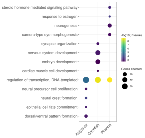
\includegraphics[width=1\textwidth]{Figures/astyanax/Go_acc_regions}
\caption[GO of ARs]{Dot plot illustrating the GO enrichment of the genes that are nearby CREs with ARs inside (putative enhancers with accelerated evolutionary rate). On the X-axis, species in which ARs have been computed. On the Y-axis are represented enriched GO terms. The dot size is proportional to the number of genes in the comparison corresponding to that GO term. The colour of the dots varies with the $-log10(PValue)$ of the enrichment. }
\label{fig:astmex_acc_regions_GO}
\end{figure}




\part{Discussion}
%Things to discuss:
%- Check the polymorphism in the surface population.
%- Main drivers of the events: ATACseq elements with a lo0t of changes?
%- Why is Astyanax the only species to do this in their caves? See if they are sharing ecosystem with other species. Related to this, which are the mechanisms that explain that. For example, there can be some molecular mechanism that marks regions in the genome and can not be repaired properly. Check the paper of the metilation to see if you can see something in this line. Also check Bilanzija work of the surface that she puts in the dark to see if there is some triggering of the phenotypic plasticity. This will be the base of your discussion, some papers that I have found: \parencite{bilandzija_phenotypic_2020, gore_epigenetic_2018, behrmann-godel_phenotypic_2023, moran_energetic_2015, uller_developmental_2018}
%- Check the GRN of the elements that are under change. This can give insight in which TFs are actually the main drivers of the adaptation. klf genes seems to be important: \parencite{gautam_multi-species_2021}. Also take a look a this paper that Rafa sugested: \parencite{ferrandez-roldan_cardiopharyngeal_2021}
%- Check reparation genes. This is ligated with the previous question, because this could explain the relationship between regulation and mutation. Eg: Methilation is altered and the repairing machinery is not able to repair some regions properly IDK.

%CHECK \parencite{bian_clock1a_2017} FOR THE DISCUSSION.: This may be related to the fact that we find some medodermal changes in cavefish, which has clock Tf alterations. Only bhle40 is affected it appears.

%check: \parencite{yoshizawa_neural_2018} you may want to use Neural crest mess up in the astyanax.
%- Check what is the enhancer that changes in otx2a, and try to find the one that explains the main change in this gene. Look for broken regulatory loops in those enhancers (maybe this would be answered when you do the ananse of the mutated regions). Functional assay???

%- Well check the QTL papers \parencite{warren_chromosome-level_2021} in order to put in context your cavefish results. Use some papers that do not explain well the mechanisms of why the genes are important to use the context of these papers with your results \parencite{leclercq_evolution_2022, ma_hypomorphic_2020}. In the latest one you have an ATAC with SNP and also nearby an accelerated region. Use this joinded result in order to explain the necesity of your data, and how they resolve some questions in the field (this is very nice cabeza).
%- The key thing is that we know many of the mechanisms that drive to the phenotypes that we see from the literature, but what we don't know is why are they happening at the same time, and in a such short amount of time.




\chapter{The effect of GRN connectivity in vertebrate body plan novelties}


Although comparing gene regulation at great evolutionary distances is challenging, it can provide insight into how morphological novelties have arisen. We used amphioxus as a proxy for the chordate ancestor and zebrafish as a vertebrate model to investigate how changes in gene regulation have contributed to the emergence of vertebrate morphological novelties. We have investigated these changes in gene regulation by altering key conserved developmental signalling pathways in amphioxus and zebrafish embryos and then analysing the transcriptomic and epigenomic consequences of these alterations (\ref{sec:Interconnectivity_chapter}). 


Transcriptomic and epigenomic data derived upon pharmacological treatment of amphioxus and zebrafish embryos revealed alterations in several genes expression and accessibility of CREs. Among other affected genes, we found many known effector genes of the treated signalling pathways. In accordance, the biological processes controlled by the affected genes were also under the control of the treated signalling pathways. For example, when disrupting FGF and Wnt pathways, we found that several mesodermal processes were affected, like somitogenesis. Indeed, these signalling pathways are known to specify and control mesodermal development \parencite{kiecker_molecular_2016}. Similar results were obtained for all treatments. When we examined the effect upon Nodal treatment, Nodal antagonists (\textit{lefty} genes) were affected, disturbing the development of mesendodermal structures like the gut. These results are in concordance with the literature, where the role of these signalling pathways in Dorso-Ventral axis patterning in embryos has been extensively described  \parencite{kiecker_molecular_2016, tuazon_temporally_2015}. Moreover, we observed that these processes were affected in both amphioxus and zebrafish, remarking on the evolutionary conservation of these signalling pathways between chordates \parencite{babonis_phylogenetic_2017}. Although the treatments affected similar functions in both species, there were some interesting differences. In zebrafish, the number of genes affected by the treatments was larger than in amphioxus, and they were more related to development. On the contrary, in amphioxus, the affected genes were more closely related to metabolism. This increase in developmental genes responding in zebrafish indicates that, in the transition from invertebrates chordates to vertebrates, these signalling pathways have gained control over more developmental processes. 


Next, we examined the response of orthologous genes between the two species to evaluate whether there is a conserved regulatory logic operating on those. We found that orthologue genes affected similarly by the same treatment tended to be developmental. Overall, we observed that several orthologue genes responded similarly to the same treatment. For example, after RA treatment, the orthologues of RA receptors \textit{rar} genes were overexpressed, altering their known role in central neural system patterning in both species \parencite{bertrand_developmental_2017, kiecker_molecular_2016}. Surprisingly, we found only a small overlap in orthologous genes when analysing Wnt-affected genes. This could suggest a deep rewiring of Wnt in the transition from chordates to vertebrates, which is compatible with the fact that \textit{Wnt} genes have undergone gain and losses of expression domains in the chordate lineage \parencite{somorjai_wnt_2018}. Therefore, we tend to believe that this finding is because, in zebrafish, there has been a notable increase in developmental genes under the control of this pathway.

We then investigated the effect of the treatments at the ATAC-seq level to identify which CREs were under the control of the treated signalling pathways. We identified DARs along the genome of both species responding to the treatments. Interestingly, the genomic distribution of the DARs between the two species is different. In amphioxus, CREs are located closer to genes, whereas zebrafish CREs tend to be in intergenic regions, indicating that gene regulation takes place at greater genomic distances in the latter organism. This phenomenon was first observed when comparing developmental CREs between zebrafish and amphioxus by Marletaz and colleagues \parencite{marletaz_amphioxus_2018}, and our DARs follow the same dynamics since they are indeed a subset of the CREs studied in this work. We also computed TFBS enrichment in DARs in order to know the effector TFs that responded to the treated signalling pathways. Similarly to our RNA-seq analysis, we identified known TF effectors. For example, \textit{tcf} TF is a known effector of Wnt in both vertebrates and amphioxus since it is bound by $\beta$-catenin and enters the nucleus to regulate the transcription of target genes \parencite{bertrand_developmental_2017, steinhart_wnt_2018}. Similarly, when examining TFBS enrichment in DARs that arose due to the overactivation of the RA pathway, we found the nuclear receptor of RAR, \textit{RAR:RXR}, and their secondary target genes, \textit{hox} genes, enriched in these DARs in both species, demonstrating the RA signalling pathway conservation in chordates \parencite{ghyselinck_retinoic_2019}. To illuminate more complex patterns of gene regulation during the treatments, we examined how the genome-wide ATAC-seq signal clustered. We explored the function of the genes nearby these groups of DARs, and we found relatively low similarity scores between zebrafish and amphioxus clusters. This could be because, especially in zebrafish, some of the clusters responded to more than one signalling pathway, potentially affecting more functions and thus reducing the similarity scores. Another possible explanation for these low similarity scores is that the GO enrichment in amphioxus depends on the aforementioned zebrafish orthology groups. By taking the entire orthology group of the amphioxus gene of interest, we may be undermining the GO enrichment analysis in amphioxus due to the inclusion of several genes related to different functions than the original amphioxus gene. However, when using the number of gene families responding to the treatments (Figure \ref{fig:DGS_GOs_fams}), we found no inflation of amphioxus gene families responding to the treatments. We then explored how developmental processes were affected by the treatments. We found that several developmental processes, like neural development, are affected by more than one signalling pathway. Moreover, we observed that, especially in zebrafish, ATAC-seq clusters tend to respond to more than one signalling pathway, indicating that those DARs are under the control of several signalling pathways. By quantifying this observation, we could show that, indeed, zebrafish have more DARs that respond to more than one signalling pathway. Thus, in zebrafish, there is more regulatory information integrated in key developmental genes. Our findings agree with those in \parencite{marletaz_amphioxus_2018}, where it was demonstrated that developmental genes gained regulatory information in the form of CREs during the chordate-to-vertebrate transition. Moreover, our data indicate that this gain of information is also due to the gain of response to key signalling pathways.


Genes that responded at both the transcriptomic and epigenetic level (DSGs) were more abundant in zebrafish than in amphioxus. The reduced number of DSGs in amphioxus could be associated with a loss of regulatory information in this species, as it has been shown that gene losses are also an important driver of evolution \parencite{guijarro-clarke_widespread_2020}. Although we can not rule out this possibility, we are more inclined to think this difference is due to the gain of regulatory input in the chordate-to-vertebrate transition \parencite{marletaz_amphioxus_2018}. In fact, in the work of Guijarro and colleagues, when they analysed the homology groups gained and lost in cephalochordates, they did not find high levels of gaining or losing genes in this group of animals \parencite{guijarro-clarke_widespread_2020}. Considering that, we studied which genes were retained in a 1-to-1 or in a 1-to-many fashion, and we found that the level of connectivity was greater in vertebrates, regardless of these categories of genes. Even so, genes that were retained as 1-to-many showed more connectivity. These genes retained in a 1-to-many manner were characterized by having more CREs and being related to developmental functions \parencite{marletaz_amphioxus_2018}. We think that their higher connectivity reflects those characteristics and that ohnologs retained in a 1-to-many manner have acquired newer CREs, integrating more regulatory information. Adding other species to the analysis helped confirm the gain of regulatory interconnectivity in the invertebrate-to-vertebrate transition, although the experimental setups were not identical. We tested if the gain of regulatory information was due to the acquisition of novel TFBS in conserved CREs, but we could not find evidence for this. Instead, we found that the newer the CREs, the more they integrated more than one signalling pathway, indicating that the gain of regulation is through new CREs that have emerged from WGDs. This fact can help to understand why specialized genes after WGD tend to have more CREs, as was shown in \parencite{marletaz_amphioxus_2018}. In fact, many specialized genes retain only one of the ancestral expression patterns, though they are the genes that have gained more CREs after WGDs. We think that these genes are integrating several signalling and regulatory cues through these new CREs.


To understand the contribution of this increase of GRN connectivity to vertebrate morphological novelties, we used previously available scRNA-seq developmental atlas of zebrafish \parencite{farnsworth_single-cell_2020}. This data allowed us to trace the expression of highly connected genes in specific tissues. We hypothesised that highly connected genes have contributed to the increased tissue complexity needed in vertebrate morphological novelties, like paired appendages or sensory placodes. We find that, in novel tissues, highly connected genes were more expressed that lowly connected genes, reinforcing our hypothesis. It is plausible that GRNs, required in these vertebrate novelties, have been enriched in these genes. For example, in the neural crest, the gene \textit{Pax3/7} is a key gene in the GRNs that control its specification and migration \parencite{simoes-costa_establishing_2015}. In our analyses, this gene in amphioxus is lowly connected, but zebrafish orthologs have gained connectivity, and some of those integrate information from up to three different signalling pathways. Together with the work of Marletaz et al., \parencite{marletaz_amphioxus_2018}, we have demonstrated that WGDs have contributed to the generation of genes that have gained more CREs in vertebrates, likely by restricting and simultaneously specifying the expression domains of these genes. In addition, we have also observed that these new CREs integrate more regulatory information from signalling pathways. We believe that these two phenomena, expression domain restriction and gain of connectivity, have contributed to generating the necessary tissue complexity present in vertebrate morphological novelties.




\chapter{The role of gene regulation to cavefish adaptation}

In this part of this project, we have analysed the role of gene regulation in adapting to a new environment. We have used \textit{Astyanax mexicanus} as a model organism to study adaptation since it presents two different populations, the surfacefish and the cave-adapted morphotype, known as cavefish. The cavefish population presents a wide range of specific phenotypes like loss of pigmentation, loss of the eyes paired with enhanced non-visual sensory capabilities, metabolic changes, circadian rhythm and behaviour alterations \parencite{jeffery_astyanax_2020, oliva_characterizing_2022}. These phenotypes have evolved independently in cavefishes at least in two independent time periods \parencite{fumey_evidence_2018, herman_role_2018, moran_selection-driven_2023}. Accordingly,  \textit{Astyanax mexicanus} constitutes a great model for EvoDevo research, since it allows us to answer many long-standing questions in Evolutionary Biology. Understanding how \textit{Astyanax mexicanus} has adapted to the cave environment expands our knowledge of the molecular, morphological, and physiological mechanisms taking place in the adaptation to this unique environment. In this study, we used \textit{Astyanax mexicanus} to decipher the developmental and gene regulatory mechanisms in cave adaptation. 

We have performed several transcriptomics and epigenomics analyses to compare the GRNs that are different between surfacefish and cavefish. When comparing the ATAC-seq clusters between cavefish and surfacefish, we found several TFBS that were different between the two populations. Then, by integrating ATAC-seq and RNA-seq in the double-selected genes (DSG) and in combination with using ANANSE, there were a series of TFs that consistently appeared as differential between the two populations. We found that the \textit{kruppel-like factors} (klf) transcription factor family is present in several of our differential analyses. These TF factors have several functions in developing key embryonic structures, which are also important for cave adaption. For example, \textit{klf4} TF is enriched in differential ATAC-seq peaks between the two populations. When integrating ATAC and RNA-seq, we find that these TFs were also enriched in the CREs that regulate DSGs, indicating that they are important for cave adaptation GRNs. This TF is an adipogenic factor, and its over-expression induces the differentiation of preadipocytes to adipocytes \parencite{li_kruppel-like_2022}. In our analysis, the binding site of this TF is enriched in those ATAC-seq peaks that are more open at the 24hpf stage, suggesting that the increase in adipose tissue in cavefish could be due to the increase in activity of this TF, among other members of the klf family, during development. Our results pinpoint other klfs with metabolic roles involved in the developmental changes that shaped the cavefish adaption. In \parencite{xiong_early_2018}, Xiong and colleagues find that in \textit{Pachón} cavefishes, the adipose tissue develops early. This early development of fat tissue contributes to the accumulation of fatty tissue, increasing the survivability of these fishes in the cave environment. Our results suggest that the early activity of \textit{klf4} TF can explain this phenotype in \textit{Pachón} cavefish. It is plausible that additional TFs contribute to the striking metabolic differences between cavefish and surfacefish. For example, \textit{hnf4a} is a key TF that drives the GRN changes between surfacefish and cavefish. Our results agree with other studies made in \textit{Astyanax mexicanus} liver cells, which find that the targets of this TF also have differential expression between cavefish and surfacefish livers \parencite{krishnan_genome-wide_2022}. Taken together, our results and the results of Krishnan and colleagues indicate that  the GRN under the control of \textit{hnf4a} is altered, potentially generating the metabolic phenotypes of cavefish. A possible explanation for this is a change in \textit{trans} in the GRN, meaning that \textit{hnf4a} suffers changes in its expression or gene sequence, impairing its function to regulate the target genes. Indeed, this gene has been demonstrated to harbour a potentially crippling mutation \parencite{warren_chromosome-level_2021}. Krishnan and colleagues do not find gene expression changes in \textit{hnf4a} in the liver cells of \textit{Astyanax mexicanus}. In contrast, our results indicate that there are changes in the expression of this gene that could explain this GRN alteration. These contrasting results between our dataset and Krishnan and colleagues are probably due to the different tissue used for the assays, since we used whole embryo samples. Additional metabolism-related TFs with differential activity between the two populations, like the \textit{NFY}, a TF related to lipid metabolism \parencite{lu_nuclear_2015}, confirm previous findings in cavefish and surfacefish adult liver cells (Krishnan et al.). Our results help to understand how the metabolic changes in the cavefish adaptation appear during development. In summary, we demonstrate that the GRNs that control the development of the liver and other metabolism-controlling tissues, like adipocytes, are significantly altered in cavefish while adapting to the cave environment.


Besides the changes related to metabolism, in our analyses, we also detected components of the circadian rhythm, like \textit{clock} and \textit{E-Box} TFs. Cavefish present several phenotypes related to the circadian rhythm, like disrupted sleep and behavioural changes \parencite{beale_circadian_2013, moran_eyeless_2014, yoshizawa_distinct_2015}. In \parencite{mack_repeated_2021}, researchers have found that there are core elements of the circadian rhythm in cavefish which do not show the normal oscillatory transcription, like \textit{cry1a}, \textit{nptx2a} or \textit{nfil3}. However, there are also secondary components of the circadian clock, like \textit{dbpb}, that show normal oscillatory behaviour. In our DSG analysis, we were able to find all the genes related to the circadian rhythm, even the ones that were suggested to show no alterations in their oscillatory behaviour. Moreover, when we analyzed which TFs strongly influenced the adaptation to the cave environment, we identified some elements of the circadian rhythm circuit, like \textit{bhlhe40}, which lost its rhythmic transcription in cavefish. Our results can help to explain the findings of Mack and colleagues' work \parencite{mack_repeated_2021}, where they identified and studied key circadian rhythm components. They could not find sequence differences in the promoter regions of these circadian genes and thus could not explain the differences in the regulatory logic of these genes. Our results complement their findings since our ATAC-seq data can reveal the different activity of distal CREs to these genes. Indeed, several CREs outside the promoter regions of these genes change their activity when comparing surfacefish to cavefish, according to our data. Further exploration of these CREs can give insight into the mechanisms and the key players of circadian rhythm disruption in cavefish adaptation. Additionally, the disruption of cavefish circadian rhythm can lead to several phenotypes which are under the control of the biological clock. In fact, alterations in key components of the circadian rhythm like \textit{bhlhe40} are found in cavefish, where muscle development is partially impaired \parencite{bian_clock1a_2017}. Indeed, \textit{myod}, among other muscle development TFs, is one of the most influential TFs driving cavefish adaptation, according to our data. Our results can provide a potential explanation for why muscle development in cavefish tends to be more irregular in terms of timing compared to surfacefish \parencite{hinaux_developmental_2011}. We believe that the disruption of several components of the circadian rhythm in cavefish alters the muscle development of cavefish, probably generating small differences in the segmentation clock necessary to generate the somites and, thus, making their tempo more irregular between embryos in cavefish. Moreover, not only is muscle development altered in cavefish, but also adult muscle phenotypes have been reported in this population. Olsen and colleagues have studied how the disruption of the circadian clock has affected the muscle in cavefish \parencite{olsen_circadian_2023}. To do so, the researchers have addressed which genes followed a rhythmic transcription in cavefish and surfacefish generating muscle RNA-seq datasets. This approach differs from the previous study \parencite{mack_repeated_2021}, where whole-body RNA-seq was performed. Our results agree with both studies since our DSG and ANANSE analyses reveal the same as them to be altered in the cavefish compared to the surfacefish. All these results show how the adaptation to the cave environment, an environment that lacks circadian cues like daylight, has impacted circadian rhythm components, thus affecting dependent processes important for cavefish adaptation.



One of the most important phenotypes in cavefish is the loss of the eyes. Accordingly, genes related to eye development are downregulated at the 24hpf stage in our RNA-seq analysis. Furthermore, the DSGs of that same stage are also related to visual perception processes. In cavefish, the degeneration process starts at around 24hpf, when first the lens gets apoptotic, and with it, the entire eye structure \parencite{strickler_lens_2007, krishnan_cavefish_2017, jeffery_astyanax_2020, devos_eye_2021}.  
Integrating ATAC-seq and RNA-seq information using ANANSE provided us with the most influential TFs behind this phenotype. Many of the TFs that are central for cavefish adaptation are those related to the eye development GRN, like \textit{vsx2}, \textit{sox}, \textit{irx7} or \textit{otx2a} genes. Our ANANSE analysis, at 24hpf, showed that the most influential TF between cavefish and surfacefish is \textit{vsx2}, which plays an important role in retinal and eye development \parencite{buono_analysis_2021}. According to Buono et al. and Letelier et al., the eye developmental GRN is robust due to the redundancy of TF operating through the same CREs \parencite{buono_analysis_2021, letelier_mutation_2023}. In the latter study, they showed how mutating \textit{vsx} paralogs in zebrafish does not lead to microphthalmia phenotypes, while the same approach in medaka fish and mice does. This data indicated the robustness of the network in zebrafish and the different importance that this TF has across vertebrates. Given that \textit{vsx2} is one of the most influential TF in transitioning from surfacefish to cavefish GRNs, we believe this factor is crucial for eye development in \textit{Astyanax mexicanus}. Another possible explanation, which could complement our previous hypothesis, is that CREs that are bound by \textit{vsx2} and other TFs have suffered mutations in their sequence, impairing the binding of these TFs.
An intriguing observation was that some TFs related to eye development, like \textit{otx2a}, appeared differential at RNA-seq level already at 10hpf. A likely explanation for this is that the specification of the eye field is already altered at earlier stages. In fact, altered spatiotemporal \textit{shh} expression in the ventral midline at 10hpf cavefish embryos leads to an earlier \textit{fgf8} expression, affecting the expression of downstream targets and ultimately, leading to eye morphogenetic defects \parencite{pottin_restoring_2011}. We think that these differences in early eye specification are the ones that make the downstream elements of the eye developmental GRN, like \textit{otx2a}, to be differentiated at so early stages. It is curious though, why the eye still develops until a certain point in development. The research group of Sylvie Rétaux has demonstrated that the cavefish eye normally develops in the early stages of development until the morphogenetic movements sort the telencephalic and hypothalamic cells from the optic cells \parencite{pottin_restoring_2011, devos_eye_2021}. Once the telencephalon and hypothalamus cells are separated from the optic cells, the eye degenerates without affecting other critical neural tissues. This suggests that there are developmental constraints as to when the eye can degenerate, and this is why a very "expensive" and seemingly unnecessary process still takes place in cavefish.


To investigate whether and how changes in the sequence of CREs have influenced cavefish adaptation, we used two approaches. First, we examined CREs with a single nucleotide change in cavefish in comparison to the surfacefish population to assess which TFBSs were affected by these disruptions. The most affected TFBSs were the \textit{klf} gene family, \textit{NFY}, and other TFs known as critical for cave adaptation. A similar approach applied in \textit{Astyanax mexicanus} liver cells \parencite{krishnan_genome-wide_2022} revealed CREs that are responsible for the metabolic phenotype of cavefish. Further exploration of our data also confirmed that these altered CREs were placed near genes with a high impact on cave adaptation processes, as, for example, important for retina specification genes \parencite{buono_analysis_2021}, \textit{hmx1}, \textit{sox11b} and \textit{tead3b}.

Second, we used comparative genomics to understand which CREs are under accelerated evolution in cavefish. These analyses revealed which CREs have undergone DNA changes likely to be explained by more evolutionary pressure.  Several regulatory regions suffered an accelerated evolutionary rate. Most of them are nearby genes that perform key functions in cave adaptation processes, such as olfactory placode development, neural development and several others. These processes are directly related to the different behaviour and metabolism of cavefish compared to surfacefish. Moreover, when we analysed the accelerated CREs that were present in the entire \textit{Astyanax mexicanus} species compared to other teleost species, we found that these accelerated CREs were nearby genes that could potentially help to adapt to the cave environment. This means that in the speciation event of the entire species, some variations could make this species more fit to adapt to the cave environment. A possible explanation for this is that there was some level of standing variation in the genome of the surfacefish that colonized the caves. In agreement with our results, Moran and colleagues have recently demonstrated that this mechanism has largely contributed to the parallel evolution of cave traits in \textit{Astyanax mexicanus} \parencite{moran_selection-driven_2023}. In this work, the genome of several hundreds of \textit{Astyanax mexicanus} individuals was sequenced to find what are the main drivers of parallel evolution in the genome of this fish. They found that most signatures of selection are due to the selection of standing variation in the surfacefish genome that colonized the cave. They also found that \textit{de novo} mutation signatures account for 40\% of the found signatures. In accordance, our results show that accelerated regions are present not only in the cavefish genome but also in surfacefish. Moreover, we found the accelerated selection in CREs regulating important genes for cave adaptation. Also, both studies (Moran et al. and the here-presented study) underline that most signatures for parallel selection are located in non-coding genome sequences. Although the role of \textit{de novo} mutations in the parallel evolution in \textit{Astyanax mexicanus} adaptation to the cave should also be taken into consideration, these results together suggest that the standing variation in ancestral surfacefish has been fixed in the populations that colonized the caves. These mechanisms could explain the fast adaptation of surfacefish to the cave environment \parencite{herman_role_2018}. This is a phenomenon also observed in other species, like the stickleback, in which the selection of standing variation in the populations drives the rapid adaptation to new environments \parencite{jones_genomic_2012, bassham_repeated_2018, reid_threespine_2021}.


Besides this hypothesis, other mechanisms may play a role in cavefish adaptation. We believe that developmental ATAC-seq and RNA-seq experiments are of great importance in resolving current questions in the cavefish community. For instance, many of the detected DARs are within known QTL regions related to cavefish phenotypes such as eye size and metabolism \parencite{mcgaugh_cavefish_2014, warren_chromosome-level_2021}. These modified CREs may explain the regulatory alterations necessary for cave adaptation. Although the lack of functional information limited us, the results of our study can shed light on the findings of several other studies that lack this regulatory information. For example, Leclercq and colleagues \parencite{leclercq_evolution_2022} carried out transcriptomic analyses in the early stages of development in cavefish, surfacefish and F1 hybrids of these two populations. Using this approach, they could determine which genes present variations between cavefish and surfacefish. Due to the inclusion of cavefish and surfacefish F1 hybrids in their analyses, they could determine whether the difference in gene expression was due to changes in CREs. They could do this by computing how biased was the allelic ratio of expression in these F1 hybrids. They found that \textit{rx3}, an important gene that specifies the eye field, has a differential expression due to changes in a nearby CRE. In our data, we could detect an element located 79Kb away from the promoter of this gene, which is not active in the developmental stages we studied. Nevertheless, this does not exclude the possibility of being activated at a different developmental time. We further found that this CRE is bound by TFs, for example, \textit{NFY} and \textit{bhlhe40}, which have already been demonstrated in our study to be important for cavefish adaptation. According to our datasets, this element is a good candidate for causing the differential expression of this gene described by Leclerq et al. Similarly, the \textit{otx2a} is surrounded by CREs that are differentially accessible, some of which harbour SNPs and accelerated regions. Furthermore, our data corroborate those from other studies, such as those published by Ma et al. In this study, \textit{cbsa} gene has defective expression due to changes in a specific CRE of this gene in cavefish \parencite{ma_hypomorphic_2020}. Our data showed changes in the activity of this CRE and additional CREs with differential chromatin accessibility, together with accelerated regions. Our integrative analysis constitutes a great resource for defining all the genes, associated CREs and TFs related to the cavefish specific characteristics. However, it is still one of the many steps to disentangle the cause-and-consequence regulatory cascade that has led to cavefish adaptation. 


In the future, these analyses will be key to deciphering the roles of other mechanisms in cavefish adaptation. Especially interesting to us is the phenotypic plasticity since it has been shown that surfacefish embryos raised in dark conditions can transcriptionally adapt to the new environment \parencite{bilandzija_phenotypic_2020}. The dark-raised fish also have phenotypes that resemble those of cave adaptation, like the presence of smaller eyes. The role of phenotypic plasticity in adaptation to the cave environment can also explain why \textit{Astyanax mexicanus} has been successful in colonising caves in such a short period of time. We hypothesise that this was the first line of adaptation and that as generations in the dark were growing, phenotypic plasticity evolved itself, allowing it to generate the necessary diversity that natural selection needs. As it has been recently demonstrated, other mechanisms play an important role in the genomic adaptation to the new environment, like the selection of standing variation, \textit{de novo}  mutations, but also hybridization between surfacefish that invade the caves and cavefish already present in the cave \parencite{herman_role_2018, moran_selection-driven_2023}. To test thoroughly the role of phenotypic adaptation in cavefish, it would be necessary to perform ATAC-seq and RNA-seq in dark-raised embryos and compare them to our datasets. This comparison will potentially show to what extent phenotypic plasticity plays a role in cave adaptation. 

In summary, our results have shown how gene regulation in cavefish contributes to adaptation to the cave environment. Our setup was based on whole embryo experiments, but the extent of these changes can be further explored by performing single-cell experiments. These experiments would help to determine at a greater resolution which are the GRNs that are behind all the processes of cavefish adaptation at the single-cell level. We could better understand the regulatory changes and how they ultimately affect the whole embryonic tissues.  Finally, the inclusion of other species of fishes that have undergone the same processes as \textit{Astyanax mexicanus}, like the recently discovered \textit{Barbatula barbatula} \parencite{behrmann-godel_phenotypic_2023}, will help to decipher which are the gene regulatory mechanisms that lead to this convergent evolution and which can explain phenotypic plasticity.


Our exploration of the role of gene regulation in different evolutionary processes during this thesis has revealed some important mechanisms. In the first part of this thesis, we have reinforced the idea that WGDs were key in the transition from invertebrate chordates to vertebrates. We went one step further than our previous studies. We demonstrated that not only the gain of regulatory information is important but also that how these new CREs integrate information in key developmental genes is of key importance to generate morphological novelties. In the second part of this thesis, we have revealed the impact of changes in gene regulation in the adaption to a new environment. We have demonstrated how the gene regulation of key developmental genes is altered in surfacefish compared to cavefish. Moreover, we have explored in detail the changes in CREs, and we have observed the direct impact of these changes in key developmental GRNs. This thesis adds to the great body of knowledge of gene regulation and evolution, remarking on the importance of understanding the gene regulatory mechanisms behind evolutionary novelty and adaptation.






\chapter{Conclusions}

\begin{enumerate}
    \item The disruption of conserved developmental signalling pathways and the epigenetic analyses of these alterations reveal core genes with differential regulation.
    \item These core genes have gained response to more regulatory inputs provided by conserved signalling pathways. This increase in response in these genes is translated into a gain of interconnectivity between signalling pathways in vertebrates.
    \item The WGDs of vertebrates contributed to this gain in interconnectivity since some copies of vertebrate developmental genes gained newer CREs that were able to integrate more regulatory information.
    \item The comparison of \textit{Astyanax mexicanus} populations during development reveals the modification of several developmental processes related to cave adaptation. These alterations are related to the differential regulation of key developmental genes in the cavefish population.
    \item We identified several alterations in CREs that correlate with the troglomorphic phenotypes of cavefish. We determined the implications of these changes and how they influence cave adaptation processes.
    \item We could identify CREs that change more rapidly than expected, remarking the importance of how strong selective pressure from the environment impacts gene regulation in the adaptation to this new environment.
\end{enumerate}
\part{Materials and Methods}

The results of the present work come from the computational analysis of diverse Next generation sequence (NGS) experiments. These NGS experiments and the treatment of embryos were done by other people in the lab. Although how these experiments are done is out of the scope of this computational thesis, I would like to acknowledge the people that did them. In the first part of the project, the drug treatments and NGS experiments were done by Sandra Jimenez \parencite{magri_assaying_2020}. In the second part of the project, the ATAC-seq experiments in \textit{Astyanax mexicanus} were performed by Elisa de la Calle, in Woodshole.

The explanation of these analyses ought to be reproducible and clear for all the people reading this work. In order to achieve that, the scripts used for computational analysis had been deposited in \href{https://github.com/alexgilgal/Thesis_methods}{this GitHub repository}.


\chapter{Computational Analysis}

In this chapter, we will explain the computational methods that have been used to produce the Results. Since computational methods are constantly evolving, there have been several iterations in how the data was analyzed, and it may vary in some details from one project to the other. In order to address this problem, we have generated a GitHub repository in which the main analyses have been posted. During this chapter, we will refer to it several times. The steps of those pipelines will be explained in detail. 

In the next table, there is all the information about genomes and gene annotations used for mapping RNA-seq or ATAC-seq.

\begin{center}
\begin{tabular}{ |c|c|c| } 
 \hline
 Species & Genome Assembly & Source \\
 \hline
 \textit{Branchiostoma lanceolatum} & Bl71nmer & \href{http://amphiencode.github.io}{Amphiencode }\\ 
 \textit{Danio rerio} & danRer10 & \href{http://hgdownload.soe.ucsc.edu/goldenPath/danRer10/bigZips/}{UCSC} \\
 \textit{Astyanax mexicanus} &  (AstMex2) & \href{http://Feb2023.archive.ensembl.org/Astyanax_mexicanus/Info/Index}{ENSEMBL}\\
 \textit{Xenopus tropicalis} & xenTro10 & \href{http://hgdownload.soe.ucsc.edu/goldenPath/xenTro10/bigZips/}{UCSC}\\
 \textit{Ptychodera flava} & Pfla1 & \href{http://octopus.unit.oist.jp/HEMIDATA/pfl.genes.gff3.gz}{Hemidata}\\
 \hline
\end{tabular}
\end{center}

\section{ATACseq}

\subsection{From raw fastq files to data visualization}

We have used two sets of files, one for each chapter of the Results of this thesis. 
\begin{itemize}
    \item The first set of data corresponds with the analysis of amphioxus and zebrafish developmental pathways, and their pharmacological disruption. These experiments consist of samples proceeding from embryos treated at 30\% of epiboly until stage 80\% of epiboly. Embryos were treated with four different sets of pharmacological compounds which affect key developmental signalling pathways. Each treatment has two replicates of ATAC-seq. In total, we have eight samples per species.
    \item The second set of data corresponds with the study of gene regulation and its impact on the cave adaptation in \textit{Astyanax mexicanus}. In this case, we have four different developmental stages in both surfacefish and cavefish. These stages are 80\% epiboly, five somites (5ss), twenty-four post fertilization (24hpf) and forty-eight hours post-fertilization (48hpf). In total, we have eight samples per population.
\end{itemize}

We developed a pipeline in order to process in a consistent manner the ATAC-seq raw data. For both sets of data previously mentioned, this pipeline was used. This pipeline can be found in the GitHub repository in the folder ATAC-seq, under the name \path{ATAC_pipe.pl}. This pipeline consists of the next steps:
\begin{itemize}
    \item Mapping of reads: Reads were mapped against the reference genome using Bowtie2 \parencite{langmead_fast_2012}. The reference genomes used were danRer10 (zebrafish), Bl71 (amphioxus), and AstMex2. Reads pairs that had an insertion length larger than 2kb were filtered out. The result of this step produces a bam file with aligned reads.
    \item Filtering and centring of reads: Reads stored in the bam file are transferred to a temporal BED file. Those reads whose insert size was less than 130 bp were marked as nucleosome-free reads and were kept. The Tn5 cut position was established moving the start of the reads -4 bp in the reverse strand and +5 bp in the forward strand. This position was extended by 5 bp in both directions. This step resulted in a BED file with those positions.
    \item Transformation of BED to BigWig. The cut positions stored in the BED were extended to 100 bp. These extended reads were used by the wigToBigWig tool to transform the BED file into a BigWig file that could be loaded in any genome browser. In our case, it was the UCSC genome browser. 

\end{itemize}

The resulting files of the \path{ATAC_pipe.pl} were used for identifying open chromatin regions in the corresponding genomes. In our case, ATAC-seq peaks were identified using IDR \parencite{li_measuring_2011}. Briefly, this method allows us to account for biological replicates in a sequencing experiment and allows us to get the set of peaks that are consistent between our replicates. The resulting BED files from the previous pipeline are fed to the \path{idr_ATAC_script.sh}, which can be found in the GitHub repository. This script will generate several files, but the one that interests us the most is the one that contains the consensus peaks between replicates. Once we have this BED file, we will have one set of peaks for each of our conditions. These bed files can be uploaded to the browser in order to visualize the open chromatin regions in the corresponding genome.

\subsection{Differential analysis of ATAC-seq}

Differential analyses were carried out using the R package DESeq2 \parencite{love_moderated_2014}. Due to the requirements of this package, ATAC-seq data has to be preprocessed in order to compute these analyses. The preprocessing of this data consist of the following steps, performed with the bedtools suit \parencite{quinlan_bedtools_2010}. 
\begin{itemize}
    \item The first step consists of the aggregation of all the peaks of the samples that will be analyzed. We will merge all the IDR peaks of the different samples in a unique BED file, which will contain all the open chromatin regions across all samples. 
    \item The second step consists of the mapping of the ATAC-seq reads to this BED file, in order to get a quantification of how many reads are inside these peaks for each sample. This will produce a BED file for each of our samples (including replicates). All these BED files will have the same number of peaks.
    \item The third step formats the resulting BED files from the previous step in a DESeq2-friendly way. We need to keep only two columns for each sample, the peak ID and the quantification. With this final step, the resulting txt files have the same format as HTSeq files, which are readable directly by DESeq2.
\end{itemize}

Provided the unimodal quantitative nature of ATAC-seq data, we used DESeq2 to infer differentially accessible regions of open chromatin. An example of this is given in the GitHub repository (\path{ATAC_deseq2.R}). We have used a Benjamin-Hochberg $P value < 0.05 $ as a cutoff for the statistical significance of differential peaks. Using this script will provide the user with several results files. This script will write a table with the differential results in a table which contains all the statistical information extracted from DESeq2. Separately, there will be two BED files, which correspond to the genomic positions of the differential peaks, under and overexpressed. These files will be used in the following steps.

\subsection{Motif enrichment}
\label{meth:motif_enrichment}

Given a set of ATAC-seq peaks, we can compute which TFBS are enriched in that set of peaks. For this, we can estimate the probability of finding a given TFBS inside a specific set of genomic regions. This probability is compared to the probability of finding this motif in a background set of genomic regions, and then we can compute the enrichment of the TFBS in the specific set of regions. In the case of the differential peaks, we take the over and underexpressed set of peaks and compute the TFBS enrichment in both cases. This is done using the HOMER tool suit \parencite{heinz_simple_2010}. We used the findMotifGenomes.pl tool, providing as a genomic background the complete set of ATAC-seq peaks which we have tested for differential expression. We have taken into account for enrichment only vertebrate motifs. The GitHub repository contains a script that analyses the necessary inputs with fixed parameters in order to preserve reproducibility. This script can be found in the ATAC-seq folder under the name \path{homer_enrichment.sh}. The resulting plain text tables and HTML tables are used for interpreting results. In some cases, when we have combined the outputs of HOMER, we need the txt files to plot the combination in a dot plot. This dot plot is produced with the script \path{combine_Homer.R}. In the end, this script produces a dot plot in which the X axis are the samples and the Y axis are different motifs. The dot size represents the enrichment score and the colour of the significance of that enrichment.

\subsection{Assigning of target genes to each ATAC-seq peak}

Peak gene association is one of the most critical steps after ATAC-seq data analysis. This is not a trivial task, but one extended practice in the field is to assign the closest genes to the peaks. We keep two genes upstream of a peak and another two downstream of it. We then filter out those assigned genes more than 1 Mb away from the ATAC-seq peak. The reason to keep genes upstream and downstream is to avoid leaving unassigned genes for each of the peaks. 

We also used GREAT \parencite{mclean_great_2010} as an alternative method for assigning genes to peaks. Briefly, the GREAT method assigns a fixed region around the TSS of a gene, in which whatever peak that falls within, will be assigned to that gene. These regions are known as basal regions. Afterwards, an extended region is computed for each gene, in which the basal region is extended until it reaches 1 Mb or overlaps with another basal region of another gene. Basal regions can overlap between them, but an extended region can not overlap with the basal region of another gene. 

The results of both methodologies, GREAT and closest gene, are overlapping, and the choice of one over the other do not alter the results in a significant way. 

As a result of both methods, we obtain a list of genes assigned to peaks. This will output will be used for integrating ATAC-seq and RNA-seq, which is discussed in detail in the section \ref{sec:integration_atac_rna}. Furthermore, the resulting gene list can be analyzed. In our case, we have computed Gene Ontology enrichment analysis. How we did it is discussed in the next section, in \ref{sec:RNAseq}.

\subsection{Clustering of ATAC-seq signal}

In both chapters of the results, we have used ATAC-seq signal clustering as a powerful tool to see differences between our samples. These clusterings were produced using Deeptools \parencite{ramirez_deeptools2_2016} and seqminer \parencite{ye_seqminer_2011} software. The computation of the cluster was done in seqminer, where we provide the BigWigs files. This software uses k-means clustering, a supervised clustering algorithm that needs the user to establish the number of clusters that will be computed beforehand. We used 12 clusters, but we kept the most representatives. The resulting clustering was then exported to a BED file which contained the positions for each cluster of peaks. This BED file was then fed to deeptools in order to generate the visualization of these clusters.


\subsection{Discovering mutations that disrupt TFBS in ATAC-seq data}

We used CRISP software \parencite{bansal_statistical_2010} in order to obtain the ATAC-seq regions that have mutations. CRISP is a software whose main function is to call variants from NGS data. The script used in order to produce this analysis was deposited in the GitHub repository. This program needs as input the following files:

\begin{enumerate}
    \item The aligned reads of ATAC-seq samples in BAM file. These BAM files were processed by the $MarkDuplicates$ tool from the Picard toolset. The parameters for this processing step are in the script deposited in GitHub.
    \item The reference genome to which the samples were mapped. In our case, this was the AstMex2 genome (surfacefish genome).
    \item The set of genomic regions the user wants to interrogate in BED format. In our case, this was all the ATAC-seq regions detected across all ATAC-seq samples.
    \item A TXT file that indicates to what sample corresponds to each BAM file. The TXT file used for our analysis has been deposited in GitHub.
\end{enumerate}

The output of CRISP was a VCF file which contained the variations detected. This VCF file was filtered in order to keep only those variants that were specific to cavefish. The script used for this filtering is deposited in GitHub. The filtered VCF was intersected with ATAC-seq peaks using $bedtools intersect$. 

In order to know if these mutations affected TFBS inside ATAC-seq peaks, we used the R package MotifBreakr \parencite{coetzee_motifbreakr_2015}. This package takes as input a VCF file, the genome in 2bit format, and a database of motifs scores. In our case, we provided the filtered VCF file, the AstMex2 genome in 2bit format and the entire JASPAR vertebrate motifs database \parencite{castro-mondragon_jaspar_2022}. The result was a table which indicated to which extent a mutation was altering the motif score in the mutated vs the reference genome

Finally, to test that the TFBS impairment was affecting the binding of TFs, we used TOBIAS \parencite{bentsen_atac-seq_2020}. This tool detects if a given TF is binding to the genome by using the fingerprint of the binding of each TF. These are the inputs that TOBIAS needs:
\begin{enumerate}
    \item A motif collection. We used the same than for MotifBreakr.
    \item The ATAC-seq BAM files. We used all our ATAC-seq samples, dividing them in cavefish and surfacefish.
    \item A genome and annotation. We used the AstMex2 genome in FASTA format and its corresponding annotation from ENSEMBL in GTF format.
\end{enumerate}

TOBIAS uses a snakemake pipeline in order to make the results reproducible. This pipeline requires the user to put the parameters of the analysis in a $config.yaml$ file. The $config.yaml$ used in our analysis is available in GitHub.

The pipeline of TOBIAS generated several folders of results. One of these outputs was how each TF is binding to the genome and if there are differences between cavefish and surfacefish in how these TF binds to the genome. We crossed this information with the results of MotifBreaker to produce the Figure \ref{fig:Motifbreakr_tobias}. This crossing of information is documented in a script in the GitHub repository.


\section{RNAseq}
\label{sec:RNAseq}

\subsection{From raw data to data visualization}

RNA-seq was used to assess the transcriptomic output of epigenetics. Just like with ATAC-seq, we have used two sets of samples for our analyses.
\begin{itemize}
    \item The first group of samples correspond to the first chapter of the results (\ref{sec:Interconnectivity_chapter}). We have the equivalent samples for Amphioxus and zebrafish as in the previous section. These experiments consist of samples proceeding from embryos treated at 30\% of epiboly until stage 80\% of epiboly. The embryos were treated with four different sets of pharmacological compounds which affect key developmental signalling pathways. We have three replicates of RNA-seq per condition. For zebrafish and amphioxus, this translates to a total of 15 fastq files (5 conditions including control with 3 replicates each of them). We also have transcriptomic information for \textit{Xenopus tropicalis} and \textit{Ptychodera flava}. In the case of these two species we only have data for two of the treatments, Nodal and FGF inhibitors. In these species, we have a total of 9 fastq files per species.
    \item The second set of samples corresponds to the second chapter of results (\ref{sec:cap_astyanax}). In this case, we used publicly available samples from the SRA archive with id PRJNA258661. This dataset consists of samples of \textit{Astyanax mexicanus} taken from embryos at different developmental points. These developmental stages are 10 hpf, 24hpf, 36 hpf and 72 hpf. There are 3 replicates by developmental stage and samples were taken from both surfacefish and cavefish (Pachón morph). 

\end{itemize}

The first step in our analysis is to assess the quality of the samples. This is done using the FastQC tool, which allows comprehensive yet easy quality control of our samples. 

Once every sample has passed QC we proceed to the mapping of the raw reads stored in the fastq files. This uses STAR aligner (version 2.5.3) \parencite{dobin_star_2013}. The reference genomes were Bl71 and danRer10 for amphioxus and zebrafish, respectively. The result of this step is a BAM file containing the mapped reads. In order to quantify the amount of reads that each gene had we have used HTseq \parencite{anders_htseq-python_2015}. For \textit{Xenopus tropicalis} and \textit{Ptychodera flava} raw samples were directly pseudo-mapped with the reference annotations of the corresponding species with Kallisto \parencite{bray_near-optimal_2016}, with default parameters. 

BAM files were transformed to BigWig using the tool bamCoverage from Deeptools. These BigWigs can be loaded into genome browsers like the UCSC genome browser.

\subsection{Differential analysis of RNA-seq}

In the case of RNA-seq, the differential analysis is more straightforward than in ATAC-seq. The quantification files produced by either Kallisto or Htseq can be loaded directly in DESeq2 for differential gene expression analysis. There is an example of this step in the GitHub repository in the RNA-seq section, \path{deseq_rnaseq.R}. In this script, we set as statistical cutoff a corrected $P value < 0.05$ and also an absolute $log_2(FC) > 1$. These parameters are a good compromise between eliminating false positive genes and keeping biological differences. 

The results of this analysis are several files containing statistical information on the differential gene expression and a list of genes that are differentially expressed between conditions. These gene lists are the ones that can be integrated with those produced in the analysis of ATAC-seq. 

In the case of amphioxus, differentially expressed genes were also translated into zebrafish genes via orthogroups. We used orthogroups as a translation layer between amphioxus and zebrafish genes. This is because we do not have a functional annotation of genes, and we want to know the orthology relationship between Amphioxus responding genes and zebrafish responding genes. In the GitHub repository, the code for obtaining this relationship can be found in \path{Amphi_zebra_fams.R}. The input of this function are the  gene IDs of amphioxus and a table containing the orthology information between amphioxus and zebrafish genes. This table of orthology contains orthogroups, or gene families, to which each amphioxus and zebrafish gene belongs. For each amphioxus gene, the function identifies to which orthogroup this amphioxus gene belongs and retrieves the entire group of zebrafish genes that belong to the same orthogroup. Since zebrafish have undergone three rounds of WGDs, one amphioxus gene can have several zebrafish orthologs. This zebrafish gene list can be further analyzed, either in order to analyse similar responses between orthologs as in Figure \ref{fig:common_affected_genes} or to compute the enriched GO terms of this set of genes.

\subsection{GO enrichment analysis}
\label{sec:GO_enrichment}

Gene Ontology (GO) analysis is a method for annotating and comparing the functions of genes based on their biological roles. It involves mapping genes to a standardized vocabulary of biological terms and concepts, known as Gene Ontology. The GO terms are organized in a hierarchical structure, allowing for a comprehensive representation of gene function at various levels of biological organization. We can compute how a certain GO term is enriched in a gene dataset. To do that, we need to select the gene universe of the analysis. In our case, these were all the genes of the organism. Next, we must provide the GO algorithm with the gene set of interest. GO enrichment is then computed by a hypergeometric test, which will compute the probability that the GO terms of the set of genes are enriched compared to the gene universe. 

In our case, these analyses were pivotal for developing both results chapters. In the GitHub repository, the script \path{GO_enrichment.R} has the necessary code for performing these analyses. These analyses were carried out using the R package TopGO. Among the several algorithms that this package provides, we used the \path{elim} algorithm. This algorithm allowed us to take into account the hierarchical structure of GO terms, selecting only the most specific ones. We selected those GO terms that accomplished a $P value < 0.05$. Take into account that P value correction is not desirable, nor doable for GO terms, since the observations are not independent (because of the hierarchy in GO structure). 

The enriched list of GO terms can be used by several different tools in order to visualize these results. One of these tools is Revigo \parencite{supek_revigo_2011}, which allows visualizing GO enrichment results as dot plots. These plots have semantical axes, meaning that the representation will cluster together GO terms that are similar.
Another way of representing these results is using a dot plot similar to the one used in motif enrichment. A script that produces these kinds of dot plots can be found in the GitHub repository (\path{dotplot_GO.R}).

Furthermore, using the GOSemSim R package, we were able to compute similarities scores between sets of GO enrichments, which gives insight into how similar are two different lists of GO terms. An example of this is represented in Figure \ref{fig:ATAC_go_similar}.

\section{Integration of ATAC-seq and RNA-seq}

\label{sec:integration_atac_rna}

We used different methods in order to integrate the epigenetic and transcriptomic information. We will describe here these methodologies for this integration and where they have been used. We will first treat the simpler approach, and then we will explain the more sophisticated one. We will also explain here how we computed connectivity scores that have led to the results of the chapter \ref{sec:Interconnectivity_chapter}.

\subsection{Integration using gene lists}

As we mentioned in the previous sections, when analyzing ATAC-seq and RNA-seq separately, we generated gene lists. In the case of RNA-seq, those lists represent the genes that are differentially expressed between conditions. On the other hand, in the case of ATAC-seq, these lists represent the genes that are close to Differentially Accessible Regions (DARs). We integrated these two sets of genes by simply computing the intersection of both lists. The result was a list of genes that are differentially expressed and also have nearby a DAR. As shown in \ref{sec:Interconnectivity_chapter}, these genes were directly changing from one condition to another, and we called them Double Selected Genes (DSGs). 

Once we obtained these gene lists, we proceeded to perform different analyses like GO enrichment, thoroughly described in \ref{sec:GO_enrichment}. We also traced back which DARs are nearby these genes in order to obtain the set of peaks that were responsible for the epigenetic response of these DSG.

\subsubsection{Computing connectivity scores for ATAC-seq and RNA-seq}

Once we integrated a gene list of genes that respond at both epigenetic and transcriptomic levels, we computed the connectivity score of the aforementioned DSGs for the first chapter of the results.

The computation of this score is a simple yet powerful tool to understand how the different DGSs are connected to the altered signaling pathways in that part of the results. Once we had the gene list of DSGs that came from each of the treatments, we counted how many treatments each of the DSGs were responding to. This connectivity score goes from one (at least the gene is responding to one treatment), up to four (the maximum possible since we have four treatments). This connectivity score was computed not only for DSGs, and can actually be computed for a given condition if we have the gene list. It was computed even with ATAC-seq regions since the genomic position can be interpreted as geneID. In definitive, we have generated a powerful tool to compute how many times a gene or genomic location is responding to different treatments. This connectivity score can be then combined with other sets of genetic information, like how many copies have been retained for each gene (Figure \ref{fig:Connectivity_genes_wgd}), or how ancient the regulatory regions are (Figure \ref{fig:DARs_connect_evolutionary_age}).


\subsection{Integration using ANANSE}

There have been several attempts to integrate the ATAC-seq signal and RNA-seq signal in order to compute GRN. The main idea behind these attempts is to know which transcription factors are binding near genes that are changing their expression, using the DNA sequence of the nearby enhancers, TFBS and ATAC-seq signal. With this idea in mind, we can build GRN of TFs affecting genes, some of which can be TFs themselves.

Under this premise, ANANSE is born \parencite{xu_ananse_2021}. We used ANANSE to understand the GRNs that are driving the cave adaptation in \textit{Astyanax mexicanus} (see \ref{sec:cap_astyanax} for details). There is a PDF guide in the GitHub repository. This guide intends to recreate our analysis of \textit{Astyanax mexicanus} in a user-friendly manner.

As input, ANANSE needs several files. It needs the ATAC-seq data in BAM format, the quantification of RNA-seq normalized by TMP (which is obtained from Kallisto), the differential analysis of gene expression, and finally, a database of the TFBS. We have followed the next steps in order to integrate ATAC-seq and RNA-seq. There are explained in much more detail in the publication of ANANSE and in the documentation of the program that can be found in \path{https://anansepy.readthedocs.io}.

\begin{enumerate}
\item \textbf{Motif database orthology.} The first step is to accommodate the TF database that ANANSE has integrated. This database has been made for human and mouse genomes, and in our case, we have used it with \textit{Astyanax mexicanus}. ANANSE developers already thought of the possibility of running ANANSE for other species, and they provided a straightforward manner to transform the database from human and mouse to our species of interest using orthology inference. The tool $motif2factors$ allows us to transform the database. We ran this tool in order to translate the database to our \textit{Astyanax mexicanus} reference genome: AstMex2.
\item \textbf{Binding.} The second step computes binding scores for each TF in the open chromatin regions. This step integrates the previously transformed database with the ATAC-seq signal. Optionally in this step, we can give ANANSE the set of regions to be examined to TF binding. If not provided, ANANSE will identify peaks from the ATAC-seq BAM file, and it will use those peaks as regions of interest. As a result of this step, we obtain an h5 file which contains the computed binding score of each TF to all the interrogated regions. In our case, we used the IDR set of peaks as regions of interest for the 24hpf ATAC-seq of both surfacefish and cavefish.
\item \textbf{Network.} The third step needs as input the binding scores resulting from the previous step and the gene expression information in TPM. This step integrates the binding information with gene expression, and thus, here is where RNA-seq and ATAC-seq information is actually integrated. In this step, ANANSE computes an interaction score between TFs and target genes. This interaction score integrates the binding score of the TF, the distance of the enhancer to the target gene, the gene expression of the TF and the expression of the target gene. As a result of this step, we obtain an interaction list, which is ordered by the interaction score.
\item \textbf{Influence.} The fourth and final step is computing influence scores.  In this step, ANANSE can compare two different conditions (networks computed before). When comparing the networks of two conditions, ANANSE is able to extract which TFs are driving the transformation of the "source" network to the "target" network. In our case, we have used it to infer the GRN that drives the adaptation to the cave environment in cavefishes. The result of this step is a list of TFs and their influence score, which measures how important the TFs are for moving from one condition to another.
\end{enumerate}

\subsubsection{Using $seq2science$ in order to automatize preprocessing of data}

We want to address that a great amount of analysis can be automatised for all the samples that we have used. In fact, the last analysis done with ANANSE used data preprocessed by pipelines, like the aforementioned seq2science. There are several pipelines, but we find this one especially interesting because of genome management. This pipeline allows for custom installation of genomes from different sources like Ensembl, UCSC and NCBI, along with gene annotations, using the $genomepy$ tool.

In our case, we have installed the AstMex2 genome using $genomepy$ and preprocessed the ATAC-seq and RNA-seq data using the pipelines available in seq2science. This allowed us to easily obtain the necessary inputs for ANANSE, like the motif database, gene expression in TPM, ATAC-seq bams and differential gene expression. The parameters and options for the pipeline were the default for both analyses. The results from these pipelines are deposited in GitHub.

\section{Comparative genomics}
\label{sec:comp_genomics}
For our evolutionary analyses, it has been key to use comparative genomics and genome alignments as tools. Here we will describe how we have used different tools in order to obtain evolutionary insights from epigenomic and transcriptomic data.

\subsection{Genomics aligments}

The generation of genomics alignments was done using Progressive Cactus \parencite{armstrong_progressive_2020}. Progressive Cactus is a reference-free genome aligner, which has allowed researchers to align hundreds of vertebrate genomes efficiently. We used this program in order to align several teleost fish genomes, including both morphotypes of \textit{Astyanax mexicanus}. We included the next species in our genomic alignment of teleost fishes: \textit{Astyanax mexicanus} both morphotypes, \textit{Danio rerio} (zebrafish), \textit{Clupea harengus} (Atlantic herring), \textit{Oryzias latipes} (medaka), \textit{Esox lucius} (Northern pike), \textit{Pygocentrus nattereri} (red-bellied piranha), \textit{Pangasianodon hypophthalmus} (striped catfish), \textit{Electrophorus electricus} (electric eel), \textit{Sinocyclocheilus grahami} (golden line barbel), \textit{Ictalurus punctatus} (channel catfish) and \textit{Colossoma macropomum} (tambaqui). In the GitHub repository, we have included a file (\path{Genome_sources.txt}) with detailed information about where those genomes were obtained and the version used. These genomes were retrieved in FASTA format, and the headers for the chromosome names were cleaned in order to obtain simple chromosome names in all the FASTA files, using the script that is available in the GitHub repository. Finally, Progressive Cactus needs as input a species tree in Newick format. A graphical interpretation of this tree is present in Figure \ref{fig:methfig_species_tree}. In this tree, we can observe that we have selected species that are close to \textit{Astyanax mexicanus}. This is because we needed to use close evolutionary species to our species of interest to obtain micro-evolutionary insights from the alignment. This will be clarified in the explanation of the next steps of the analysis.

\begin{figure}
\centering
\includegraphics{Figures/astyanax/species_tree}
\caption[Species tree used for comparative genomics]{Species tree used for comparative genomics.}
\label{fig:methfig_species_tree}
\end{figure}

Once we provided all the necessary input for Progressive Cactus, the program started to align the different genomes in a referenceless manner. This process was the most computationally intense in this thesis since the process took one month to finish. Once the alignment was finished, the result was an alignment file in hal format. The Cactus toolkit allows the transformation of this hal file to a given set of alignment standard formats, giving a reference. We exported the alignments to MAF alignment files which can be read by downstream tools.

\subsection{Accelerated regions}

Once we produced the MAF files from the alignment, we started to use standard comparative genomics tools. One that has been key to understanding how \textit{Astyanax mexicanus} has adapted to the cave environment has been PHAST \parencite{hubisz_phast_2011}. Using these tools, we were able to compute regions that show an accelerated evolution ratio compared to other genomic regions. This analysis used several scripts, which can be found in GitHub under the folder \path{Comparative_genomics}. I strongly encourage the reader to check the vignettes in the \href{http://compgen.cshl.edu/phast/resources.php}{PHAST web page} in case he/she need to perform these analyses. We used the R interface for PHAST, the package rphast for these analyses. An R script can be found in the GitHub repository with the code that we used.

In the first place, we computed those intergenic regions that were conserved between all the species in the alignment except our species of interest. In our case, this translates to using all the genomes for this computation but the cavefish one. This is because we used these regions as a "baseline" for variation in our data. Hence, we could not use the species we tested for computing this baseline.

Once we computed the conserved regions, we calculated which regions were accelerated. In this step, we used the complete alignment with all the species. We kept those conserved regions that fulfil the following conditions:
\begin{enumerate}
    \item Regions have to be present in cavefish since it is our testing organism.
    \item Regions need to appear in at least five species.
    \item Regions need to be present in species that are close to cavefish. These species are Surfacefish, piranha, electric eel, and both catfish and tambaqui.
\end{enumerate}

Once we selected these candidate regions, we computed the acceleration rate in Cavefish, using the function phyloP from rphast package. The problem with this tool was that it does not compute statistical significance for the regions. We used an empirical approach to compute this P value, and that was done by using random alignments and comparing the distribution of acceleration in real data vs simulated random data. Once we did this, we selected those regions with a corrected $P value < 0.05$. The $P value$ was corrected using Benjamin-Hochberg. Finally, we wrote the resulting accelerated regions into a bed file.

Note that this analysis can be done for several species, as long as we compute conserved regions without the species of interest. We did this analysis not only for cavefish but also for the entire \textit{Astyanax mexicanus} species and for piranha. Once we obtained the BED file with accelerated regions, we performed several analyses with them. We crossed these regions with ATAC-seq peaks and perform the aforementioned analyses in the previous sections (\ref{meth:motif_enrichment}).

%----------------------------------------------------------------------------------------
%	THESIS CONTENT - APPENDICES
%----------------------------------------------------------------------------------------

%\appendix % Cue to tell LaTeX that the following "chapters" are Appendices

% Include the appendices of the thesis as separate files from the Appendices folder
% Uncomment the lines as you write the Appendices

%\include{Appendices/AppendixA}
%\include{Appendices/AppendixB}
%\include{Appendices/AppendixC}

%----------------------------------------------------------------------------------------
%	BIBLIOGRAPHY
%----------------------------------------------------------------------------------------

\printbibliography[heading=bibintoc]

%----------------------------------------------------------------------------------------

\end{document}  